\documentclass{bbawslides}

\usepackage[TS1, T1]{fontenc}
\usepackage{ifthen}

\usepackage[a4paper]{hyperref}
\rotateheaderstrue	%%-- otherwise seminar does strange things
\usepackage{url}

\usepackage[ngerman]{babel}
\usepackage[babel]{csquotes}
\usepackage[autoplay]{animate}
\usepackage{graphicx}
\usepackage{numprint}
\npthousandsep{~}\npthousandthpartsep{}\npdecimalsign{,}

\DeclareTextSymbol{\textlongs}{TS1}{115} 
\DeclareTextSymbolDefault{\textlongs}{TS1}


\begin{document}
\providecommand{\Title}{}


\begin{bbawtitle}[(Open-Source-)OCR-Workflows]
  \vspace*{3em}%
  Kay-Michael Würzner\\[-.25em]%
  \textcolor{urlColor}{\texttt{{\small wuerzner@bbaw.de}}}
  \\[3em]
  {\footnotesize{%
    DH-Kolloquium an der Berlin-Brandenburgischen Akademie der Wissenschaften\\%
    4. August 2017\\%
  }}
\end{bbawtitle}
\slideStyleFrame

\renewcommand{\footerText}{\tiny 4. August 2017, DH-Kolloquium, BBAW}

%----------------------------------------------------------------------------------------------
% Outline
%----------------------------------------------------------------------------------------------
\begin{bbawslide}{Übersicht}
  \vspace*{7mm}%
  \centerslidestrue%
  \begin{itemize}
    \item Einleitung
    \begin{itemize}\small
      \item Was ist OCR?
      \item Wozu benutzt man OCR?
      \item Warum überhaupt OCR?
    \end{itemize}
    \item Technische Aspekte
    \begin{itemize}\small
      \item Komponenten eines einfachen OCR-Workflows
      \item Modelltraining
      \item Optimierungsoptionen
      \item Komplexere OCR-Workflows
    \end{itemize}
    \item Nichttechnische Aspekte
    \begin{itemize}\small
      \item OCR-D
      \item Open-Source, und dann?
    \end{itemize}
  \end{itemize}
\end{bbawslide}

\begin{bbawpart}{\Large\bf Was ist OCR?}
\end{bbawpart}

\begin{bbawslide}{Was ist OCR?}
  \vspace*{7mm}%
  \centerslidestrue%
  \begin{tabular}{lc}
    \begin{minipage}{0.6\textwidth}
      \begin{itemize}
        \item \textbf{O}ptical \textbf{C}haracter \textbf{R}ecognition: Automatische Erfassung von Text in Bildern
        \item ursprünglich begrenzt auf Zeichenerkennung
        \item heute häufig Synonym für den gesamten Texterfassungsprozess
        \begin{itemize}
          \item Bildvorverarbeitung
          \item Layoutanalyse (OLR)
          \item Zeilenerkennung
          \item \ldots
        \end{itemize}
      \end{itemize}
    \end{minipage}
    &
    \begin{minipage}{0.4\textwidth}
      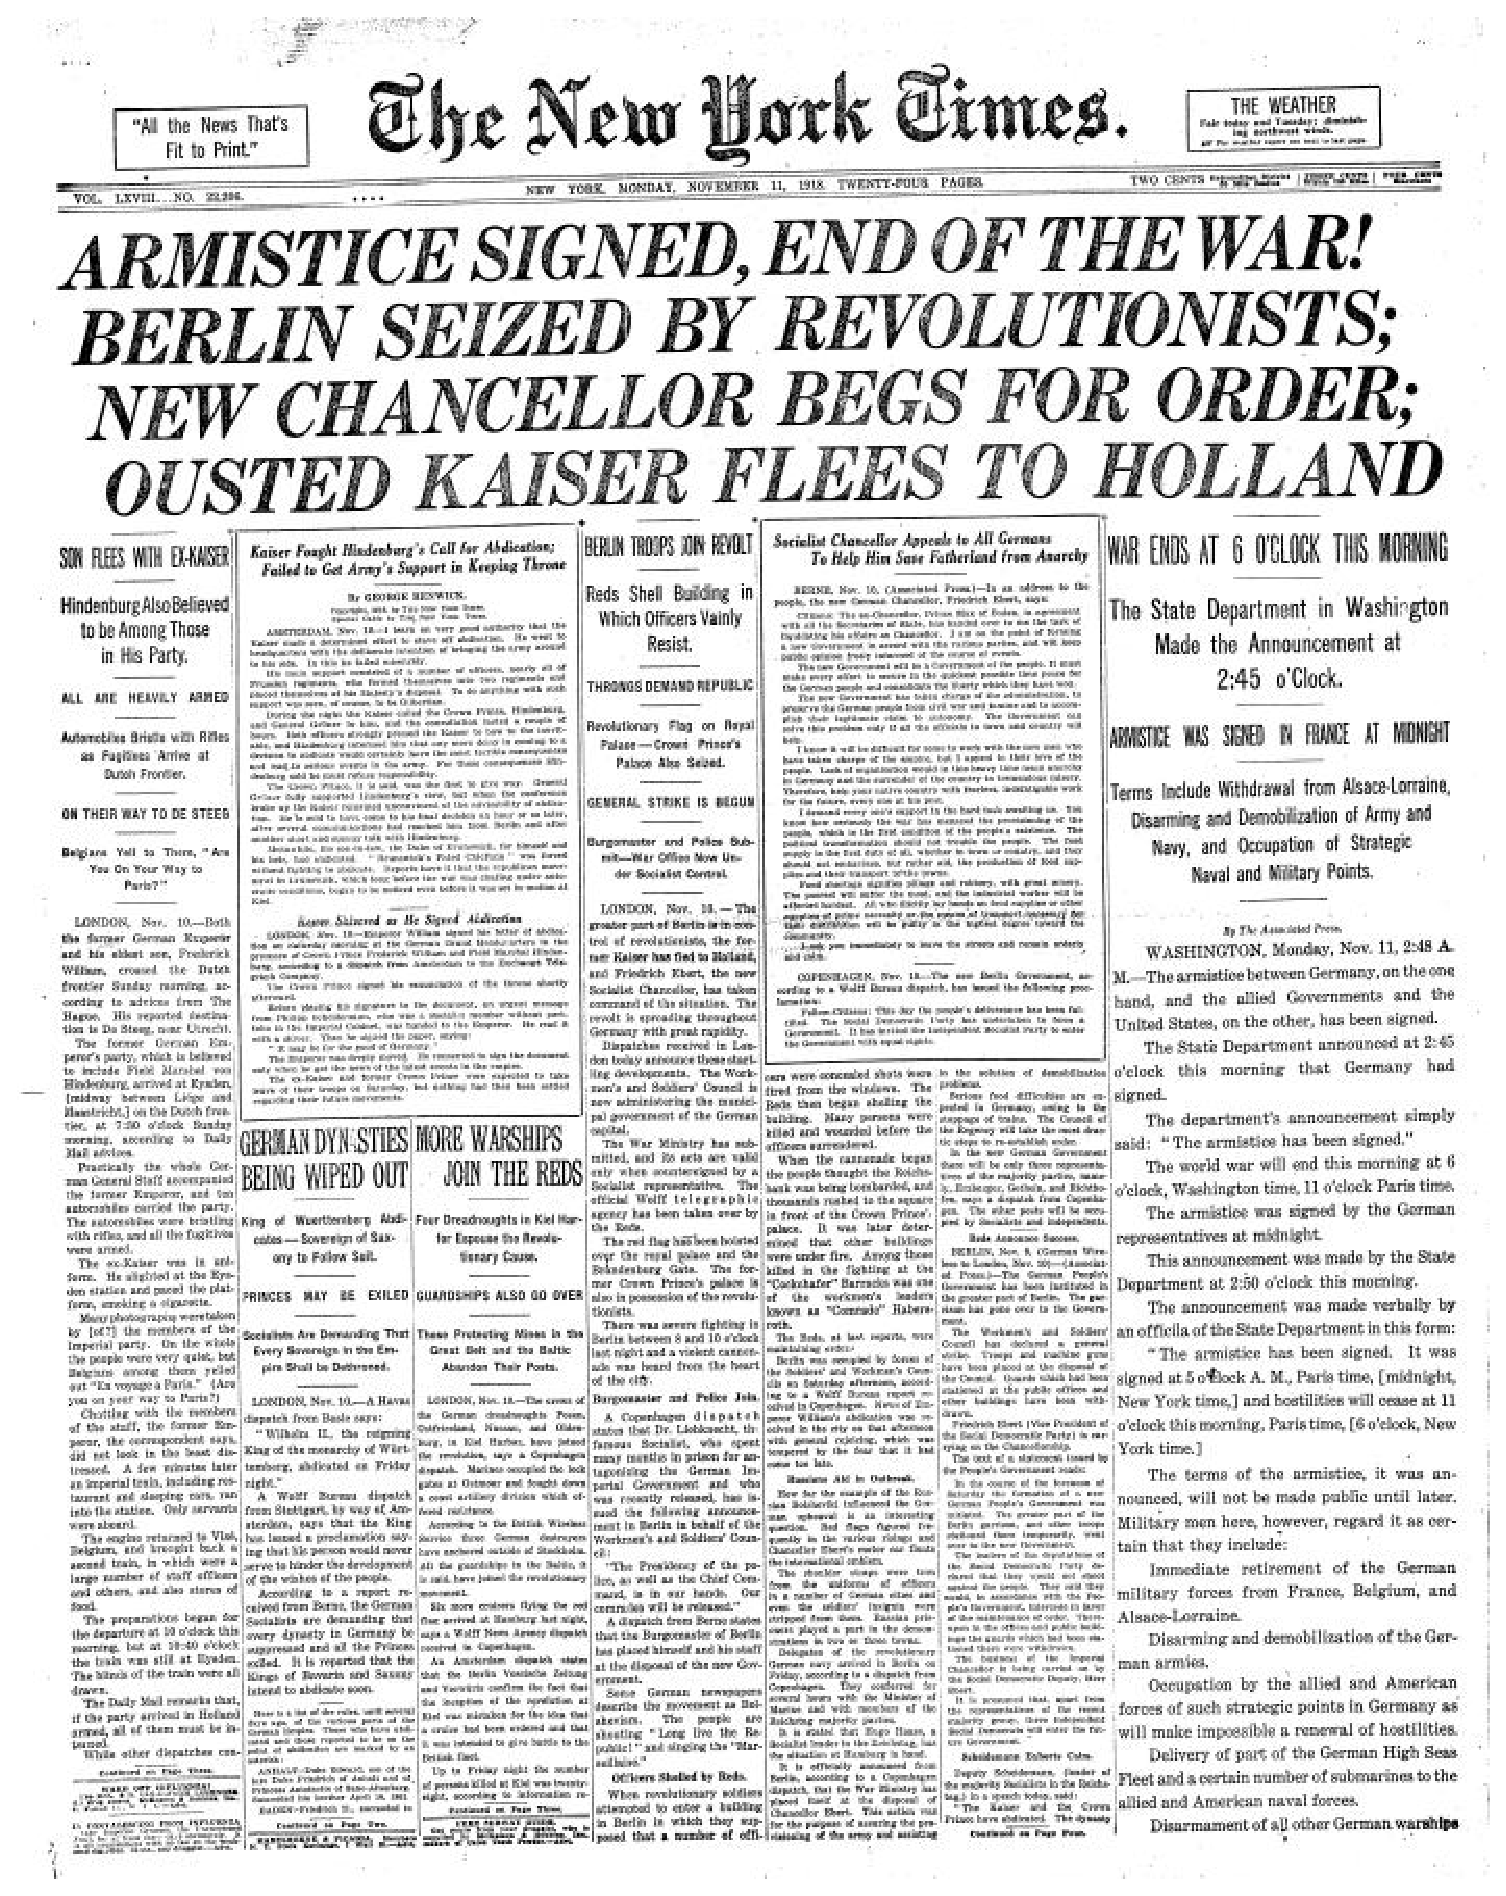
\epsfig{file=figures/times.eps,width=\textwidth}
    \end{minipage}
  \end{tabular}
\end{bbawslide}

\begin{bbawslide}{Zeichenorientierte Ansätze}
  \vspace*{7mm}%
  \hspace*{-2em}%
  \centerslidestrue%
  \begin{tabular}{lc}
    \begin{minipage}{0.68\textwidth}
      \begin{mitemize}
      \item Erkennung erfolgt \emph{glyphenweise}
        \begin{description}\small
          \item[Pattern matching:] Vergleich der Zeichenbilder zu in einem \enquote{Setzkasten} gespeicherten Glyphen \textbf{Pixel für Pixel}
          \item[Feature extraction:] Zerlegung der Glyphen in vordefinierte, bedeutungstragende \textbf{Eigenschaften}
          wie \emph{Einfärbung, Kurven, Linien} etc. und Vergleich zu Trainingsmaterialien
        \end{description}
      \item Kombination beider Ansätze möglich
      \item Zerlegung der Seite in \emph{Zeilen} und \emph{Zeichen} notwendig
      \item Open-Source Software \texttt{Tesseract 3} \hlcite{Smith 2007}
        \begin{mitemize}\small
          \item Einsatz verschiedener Lexika für frequente Wörter, Sonderzeichen und
        häufige Fehler zur Verbesserung der Erkennung
        \end{mitemize}
      \end{mitemize}
    \end{minipage}
    &
    \begin{minipage}{0.38\textwidth}
      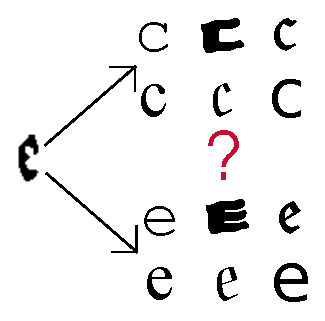
\epsfig{file=figures/char.eps,width=\textwidth}
    \end{minipage}
  \end{tabular}
\end{bbawslide}

\begin{bbawslide}{Zeilenorientierte Ansätze}
  \vspace*{7mm}%
  \centerslidestrue%
  \begin{minipage}{1.05\textwidth}
    \begin{itemize}
      \item Erkennung erfolgt \emph{zeilenweise}
        \begin{description}\small
          \item[Scaling:] Einheitliche Höhe für alle Zeilen
          \item[Feature extraction:] Grid mit festgelegter Anzahl (horizontaler) Zeilen und variabler Anzahl
                                     (vertikaler) Spalten: Zeilen als Sequenzen binärwertiger Vektoren fixer Länge
        \end{description}
    \end{itemize}
  \end{minipage}
  \begin{center}
    
\epsfig{file=figures/grid.eps,width=1.05\textwidth}
  \end{center}
  \begin{minipage}{1.05\textwidth}
    \begin{itemize}
      \item Kontextsensitive (i.e.~ über \emph{Übergangswahrscheinlichkeiten} der Vektoren) Erkennung
      \item Zerlegung der Seite in \emph{Zeilen} notwendig
      \item Vorgehen (normalerweise) \emph{robuster} gegenüber Varianz durch Artefakte als zeichenorientierte Ansätze
      \item Open-Source Software \texttt{OCRopus} \hlcite{Breuel 2008}
      \begin{mitemize}\small
        \item Einsatz \emph{neuronaler Netzwerke} für die Sequenzklassifikation
      \end{mitemize}
    \end{itemize}
  \end{minipage}
\end{bbawslide}

\begin{bbawpart}{\Large\bf Wozu braucht man OCR?}
\end{bbawpart}

\renewcommand{\footerText}{\tiny 4. August 2017, DH-Kolloquium, BBAW\hspace{4cm} Image by Achim Raschka, CC BY-SA 3.0}

\begin{bbawslide}{Wozu braucht man OCR?}
  \vspace*{1mm}%
  \centerslidesfalse%
  \begin{tabular}{cc}
    \raisebox{-\height}{\parbox{7cm}{%
      \begin{itemize}
        \item typische Anwendungen:
        \begin{itemize}\small
          \item Nummernschilderkennung (\emph{Automatic number plate recognition})
        \end{itemize}
      \end{itemize}
    }}
    &
    \raisebox{-\height}{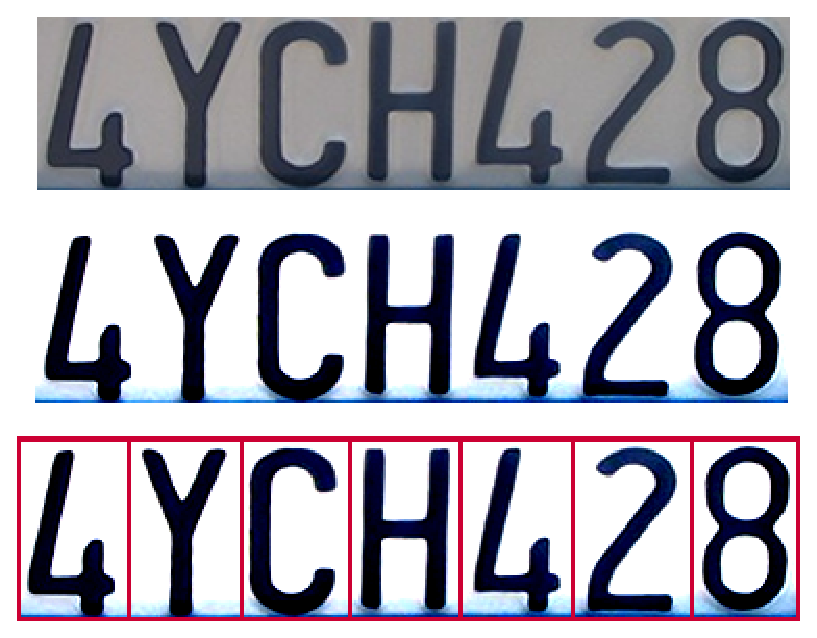
\epsfig{file=figures/ANPR.eps,width=0.4\textwidth}}%
  \end{tabular}
\end{bbawslide}

\renewcommand{\footerText}{\tiny 4. August 2017, DH-Kolloquium, BBAW\hspace{4cm} Image by JD, CC BY-SA 2.0}

\begin{bbawslide}{Wozu braucht man OCR?}
  \vspace*{1mm}%
  \centerslidesfalse%
  \begin{tabular}{cc}
    \raisebox{-\height}{\parbox{7cm}{%
      \begin{itemize}
        \item typische Anwendungen:
        \begin{itemize}\small
          \item Nummernschilderkennung (\emph{Automatic number plate recognition})
          \item Captcha-Umgehung (\emph{Completely Automated Public Turing test to tell Computers and Humans Apart})
        \end{itemize}
      \end{itemize}
    }}
    &
    \raisebox{-\height}{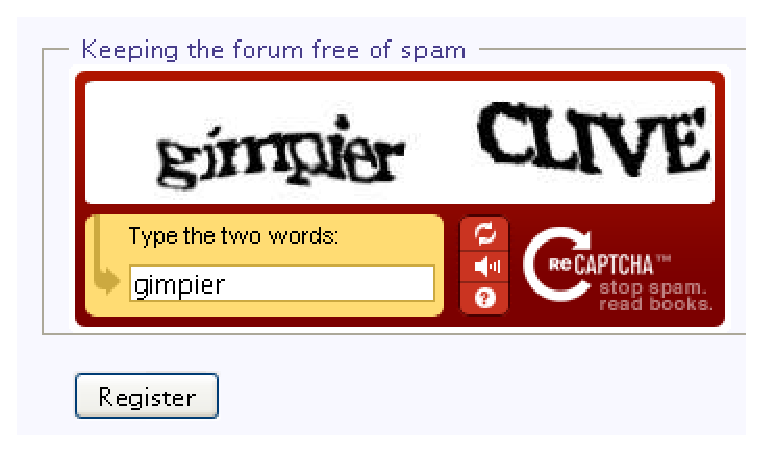
\epsfig{file=figures/Captcha.eps,width=0.4\textwidth}}%
  \end{tabular}
\end{bbawslide}

\renewcommand{\footerText}{\tiny 4. August 2017, DH-Kolloquium, BBAW\hspace{4cm} Image by Eluminary, CC BY-SA 4.0}

\begin{bbawslide}{Wozu braucht man OCR?}
  \vspace*{1mm}%
  \centerslidesfalse%
  \begin{tabular}{cc}
    \raisebox{-\height}{\parbox{7cm}{%
      \begin{itemize}
        \item typische Anwendungen:
        \begin{itemize}\small
          \item Nummernschilderkennung (\emph{Automatic number plate recognition})
          \item Captcha-Umgehung (\emph{Completely Automated Public Turing test to tell Computers and Humans Apart})
          \item Schlüsselinformationsextraktion (\emph{Document's key information extraction})
        \end{itemize}
      \end{itemize}
    }}
    &
    \raisebox{-\height}{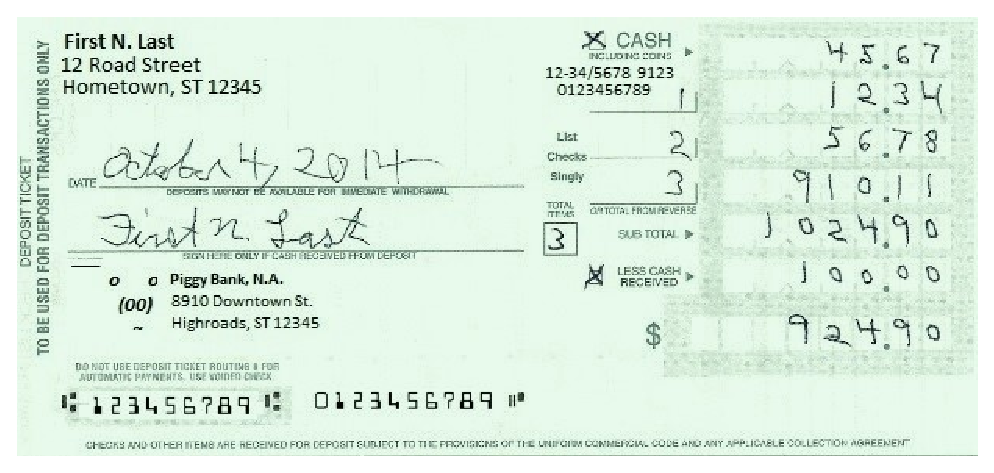
\epsfig{file=figures/deposit.eps,width=0.4\textwidth}}%
  \end{tabular}
\end{bbawslide}

\renewcommand{\footerText}{\tiny 4. August 2017, DH-Kolloquium, BBAW}

\begin{bbawslide}{Wozu braucht man OCR?}
  \vspace*{1mm}%
  \centerslidesfalse%
  \begin{tabular}{cc}
    \raisebox{-\height}{\parbox{7cm}{%
      \begin{itemize}
        \item typische Anwendungen:
        \begin{itemize}\small
          \item Nummernschilderkennung (\emph{Automatic number plate recognition})
          \item Captcha-Umgehung (\emph{Completely Automated Public Turing test to tell Computers and Humans Apart})
          \item Schlüsselinformationsextraktion (\emph{Document's key information extraction})
          \item Handschrifterkennung (\emph{Handwritten text recognition})
        \end{itemize}
      \end{itemize}
    }}
    &
    \raisebox{-\height}{\epsfig{file=figures/transkribus.eps,width=0.4\textwidth}}%
  \end{tabular}
\end{bbawslide}

\renewcommand{\footerText}{\tiny 4. August 2017, DH-Kolloquium, BBAW\hspace{4cm} Images by Uwe Springmann, CC BY-SA 4.0}

\begin{bbawslide}{Wozu braucht man OCR?}
  \vspace*{1mm}%
  \centerslidesfalse%
  \begin{tabular}{cc}
    \raisebox{-\height}{\parbox{7cm}{%
      \begin{itemize}
        \item typische Anwendungen:
        \begin{itemize}\small
          \item Nummernschilderkennung (\emph{Automatic number plate recognition})
          \item Captcha-Umgehung (\emph{Completely Automated Public Turing test to tell Computers and Humans Apart})
          \item Schlüsselinformationsextraktion (\emph{Document's key information extraction})
          \item Handschrifterkennung (\emph{Handwritten text recognition})
          \item \textbf{Volltextdigitalisierung}
        \end{itemize}
      \end{itemize}
    }}
    &
    \raisebox{-\height}{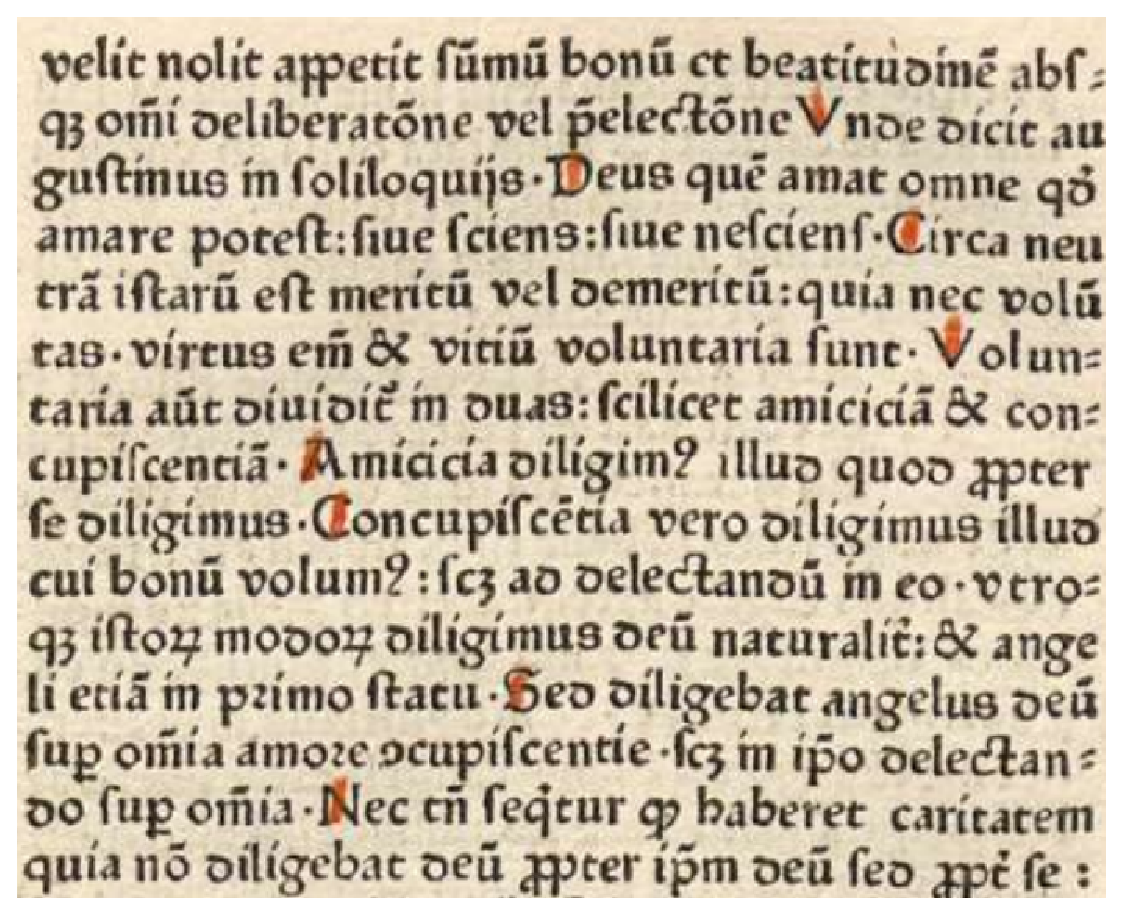
\epsfig{file=figures/beauvais_0.eps,width=0.4\textwidth}}%
  \end{tabular}
\end{bbawslide}

\begin{bbawslide}{Wozu braucht man OCR?}
  \vspace*{1mm}%
  \centerslidesfalse%
  \begin{tabular}{cc}
    \raisebox{-\height}{\parbox{7cm}{%
      \begin{itemize}
        \item typische Anwendungen:
        \begin{itemize}\small
          \item Nummernschilderkennung (\emph{Automatic number plate recognition})
          \item Captcha-Umgehung (\emph{Completely Automated Public Turing test to tell Computers and Humans Apart})
          \item Schlüsselinformationsextraktion (\emph{Document's key information extraction})
          \item Handschrifterkennung (\emph{Handwritten text recognition})
          \item \textbf{Volltextdigitalisierung}
        \end{itemize}
      \end{itemize}
    }}
    &
    \raisebox{-\height}{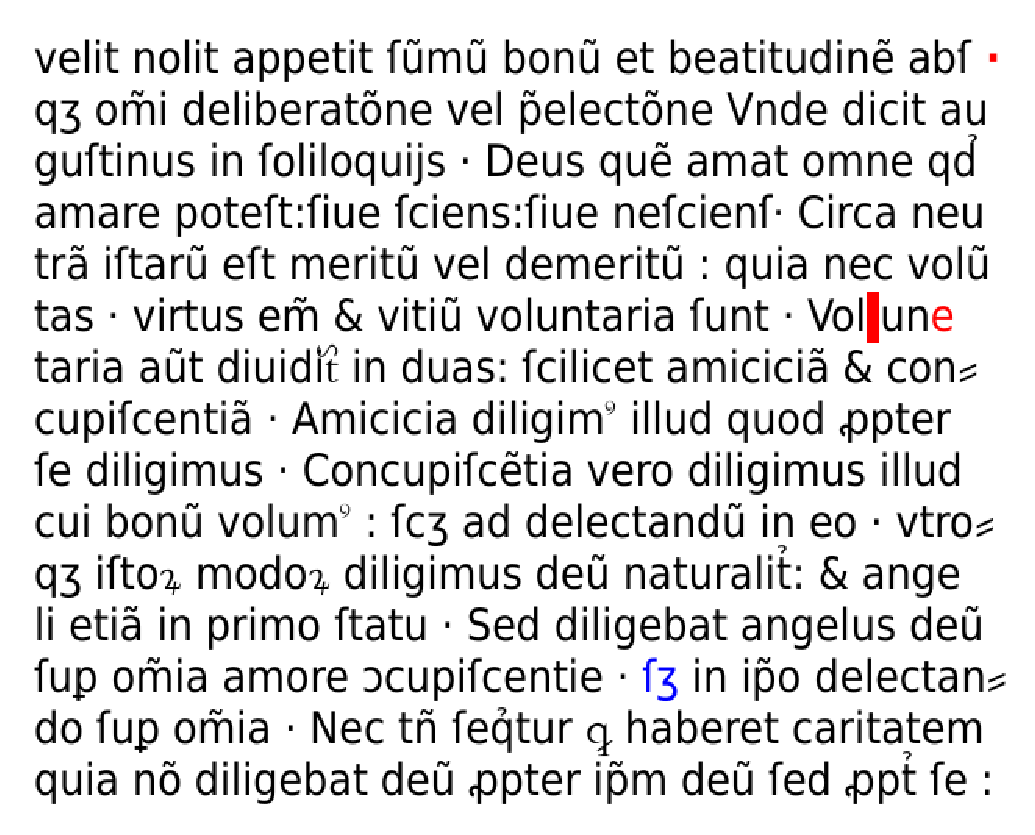
\epsfig{file=figures/beauvais_1.eps,width=0.4\textwidth}}%
  \end{tabular}
\end{bbawslide}

\renewcommand{\footerText}{\tiny 4. August 2017, DH-Kolloquium, BBAW}

\begin{bbawslide}{Warum überhaupt OCR?}
  \vspace*{7mm}%
  \centerslidestrue%
  \begin{itemize}
    \item OCR ist immer \textbf{fehlerhaft}! Aber:
    \item verändertes \enquote{Rechercheverhalten} in Zeiten zunehmender Verfügbarkeit
          digitaler Quellen
          \begin{itemize}\small
            \item Wissenserwerb durch Internetsuche
            \item Sekundärliteratur (fast) vollständig \textbf{textdigital} verfügbar
            \item Navigationssystem vs. Autoatlas
          \end{itemize}
     \item Ansprüche an Verfügbarkeit von \textbf{Primärquellen} wächst
     \item vielfältige quantitative Auswertungsmethoden (i.e.~\emph{distant reading})
     \item für den \textbf{Digital Humanist}: Bruch mit dem \enquote{Diktat der Verfügbarkeit}
  \end{itemize}
\end{bbawslide}

\begin{bbawpart}{\Large\bf Komponenten eines einfachen OCR-Workflows}
\end{bbawpart}

\begin{bbawslide}{Komponenten eines einfachen OCR-Workflows}
  \vspace*{2mm}%
  \centerslidestrue%
  \begin{tabular}{cc}
    \phantom{\raisebox{-3\height}{\parbox{7cm}{%
      \begin{enumerate}
        \item Bildvorverarbeitung
        \item Layoutanalyse
        \item Texterkennung
      \end{enumerate}
    }}}
    &
    \raisebox{-\height}{\epsfig{file=figures/grenzboten_raw.eps,width=0.4\textwidth}}%
  \end{tabular}
\end{bbawslide}

\begin{bbawslide}{Komponenten eines einfachen OCR-Workflows}
  \vspace*{2mm}%
  \centerslidestrue%
  \begin{tabular}{cc}
    \raisebox{-3\height}{\parbox{7cm}{%
      \begin{enumerate}
        \item Bildvorverarbeitung
        \item
        \item
      \end{enumerate}
    }}
    &
    \raisebox{-\height}{\epsfig{file=figures/grenzboten_raw.eps,width=0.4\textwidth}}%
  \end{tabular}
\end{bbawslide}

\begin{bbawslide}{Komponenten eines einfachen OCR-Workflows}
  \vspace*{2mm}%
  \centerslidestrue%
  \begin{tabular}{cc}
    \raisebox{-3\height}{\parbox{7cm}{%
      \begin{enumerate}
        \item Bildvorverarbeitung
        \item
        \item
      \end{enumerate}
    }}
    &
    \raisebox{-\height}{\epsfig{file=figures/grenzboten_opt.eps,width=0.4\textwidth}}%
  \end{tabular}
\end{bbawslide}

\begin{bbawslide}{Komponenten eines einfachen OCR-Workflows}
  \vspace*{2mm}%
  \centerslidestrue%
  \begin{tabular}{cc}
    \raisebox{-3\height}{\parbox{7cm}{%
      \begin{enumerate}
        \item Bildvorverarbeitung
        \item Layoutanalyse
        \item
      \end{enumerate}
    }}
    &
    \raisebox{-\height}{\epsfig{file=figures/grenzboten_opt.eps,width=0.4\textwidth}}%
  \end{tabular}
\end{bbawslide}

\begin{bbawslide}{Komponenten eines einfachen OCR-Workflows}
  \vspace*{2mm}%
  \centerslidestrue%
  \begin{tabular}{cc}
    \raisebox{-3\height}{\parbox{7cm}{%
      \begin{enumerate}
        \item Bildvorverarbeitung
        \item Layoutanalyse
        \item
      \end{enumerate}
    }}
    &
    \raisebox{-\height}{\epsfig{file=figures/grenzboten_struct.eps,width=0.4\textwidth}}%
  \end{tabular}
\end{bbawslide}

\begin{bbawslide}{Komponenten eines einfachen OCR-Workflows}
  \vspace*{2mm}%
  \centerslidestrue%
  \begin{tabular}{cc}
    \raisebox{-3.001\height}{\parbox{7cm}{%
      \begin{enumerate}
        \item Bildvorverarbeitung
        \item Layoutanalyse
        \item Texterkennung
      \end{enumerate}
    }}
    &
    \raisebox{-\height}{\epsfig{file=figures/grenzboten_struct.eps,width=0.4\textwidth}}%
  \end{tabular}
\end{bbawslide}

\begin{bbawslide}{Komponenten eines einfachen OCR-Workflows}
  \vspace*{2mm}%
  \centerslidestrue%
  \begin{tabular}{cc}
    \raisebox{-3.001\height}{\parbox{7cm}{%
      \begin{enumerate}
        \item Bildvorverarbeitung
        \item Layoutanalyse
        \item Texterkennung
      \end{enumerate}
    }}
    &
    \raisebox{-\height}{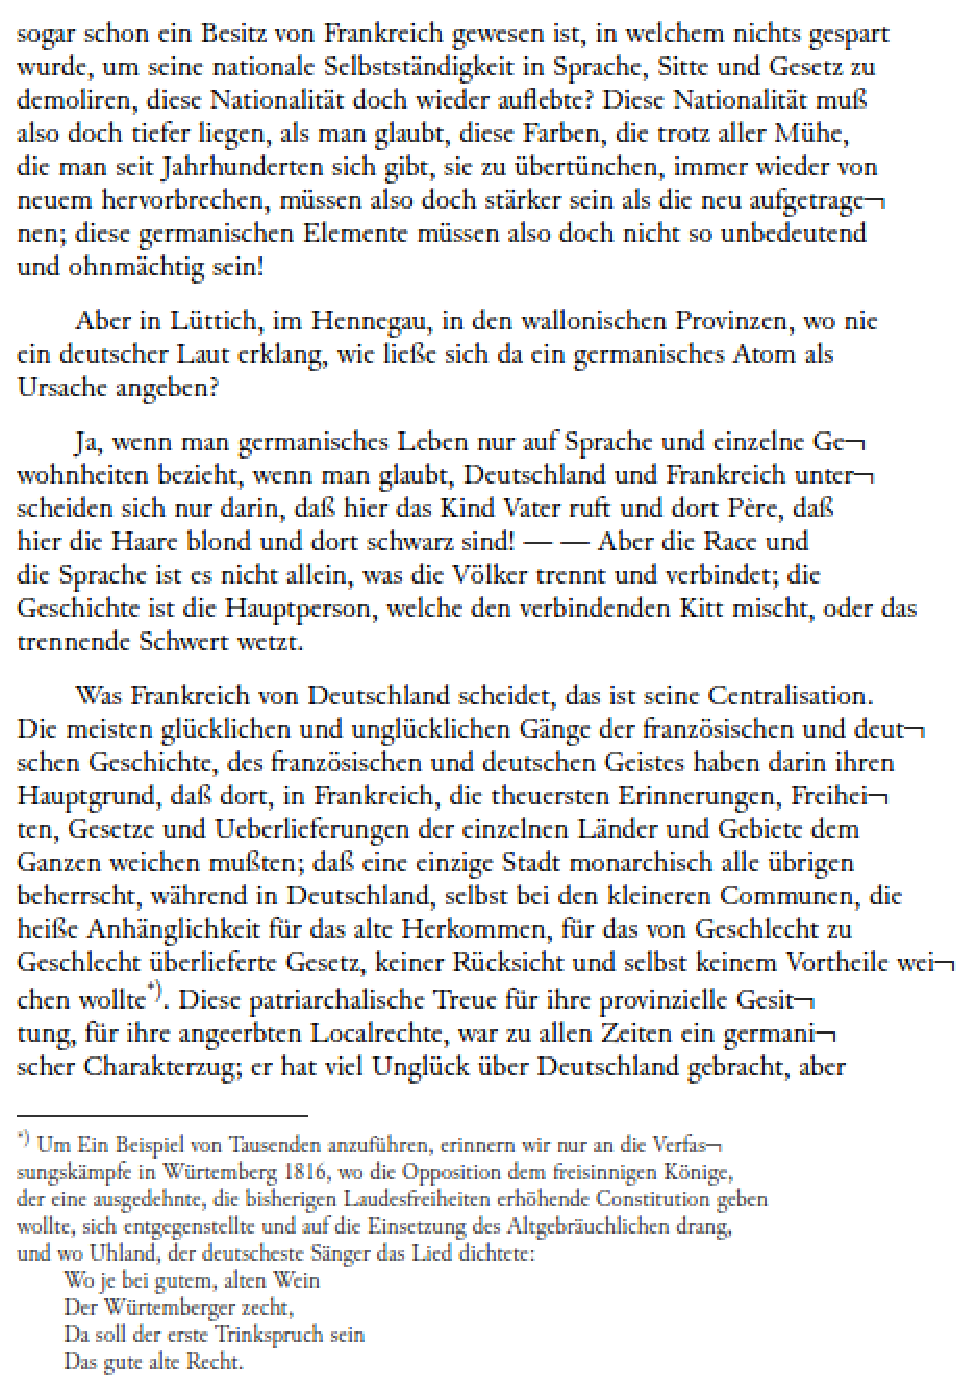
\epsfig{file=figures/grenzboten_text.eps,width=0.4\textwidth}}%
  \end{tabular}
\end{bbawslide}

\begin{bbawslide}{Komponenten eines OCR-Workflows: Bildvorverarbeitung}
  \vspace*{7mm}%
  \centerslidestrue%
  \begin{itemize}
    \item Prozesse zur bestmöglichen Vorbereitung der Digitalisate für OLR und OCR
    \begin{itemize}\small
      \item \textbf{Cropping:} Beschneidung des Digitalisats auf den Druckbereich
      \item \textbf{Deskewing:} Rotation des Digitalisats zur Begradigung von Schrägstellungen
      \item \textbf{Binarization:} Binäre Kodierung der Pixel (bedruckte Bereiche schwarz, nicht-bedruckte Bereiche weiß)
      \item \textbf{Despeckling:} Entfernung von Bildartefakten (Verschmutzungen, sichtbare Papiermaserung etc.)
      \item \textbf{Dewarping:} Begradigung von Wellen auf Zeilenebene
    \end{itemize}
    \item starker Einfluss auf die Erkennungsqualität
    \item besondere Relevanz für historische Vorlagen
  \end{itemize}
\end{bbawslide}

\begin{bbawslide}{Komponenten eines einfachen OCR-Workflows: Cropping}
  \vspace*{2mm}%
  \begin{center}
    \begin{tabular}{c@{\hspace{1cm}}c}
      \raisebox{-\height}{\epsfig{file=figures/cropping_in.eps,width=0.3\textwidth}}%
      &
      \raisebox{-\height}{\epsfig{file=figures/cropping_out.eps,width=0.3\textwidth}}%
    \end{tabular}
  \end{center}
\end{bbawslide}

\begin{bbawslide}{Komponenten eines einfachen OCR-Workflows: Deskewing}
  \vspace*{2mm}%
  \begin{center}
    \begin{tabular}{c@{\hspace{1cm}}c}
      \raisebox{-\height}{\epsfig{file=figures/deskewing_in.eps,width=0.3\textwidth}}%
      &
      \raisebox{-\height}{\epsfig{file=figures/deskewing_out.eps,width=0.3\textwidth}}%
    \end{tabular}
  \end{center}
\end{bbawslide}

\begin{bbawslide}{Komponenten eines OCR-Workflows: Binarization}
  \vspace*{2mm}%
  \begin{center}
    \begin{tabular}{c@{\hspace{1cm}}c}
      \raisebox{-\height}{\epsfig{file=figures/binarization_in.eps,width=0.4\textwidth}}%
      &
      \raisebox{-\height}{
\epsfig{file=figures/binarization_out.eps,width=0.4\textwidth}}%
    \end{tabular}
  \end{center}
\end{bbawslide}

\begin{bbawslide}{Komponenten eines OCR-Workflows: Despeckling}
  \vspace*{2mm}%
  \begin{center}
    \begin{tabular}{c@{\hspace{1cm}}c}
      \raisebox{-\height}{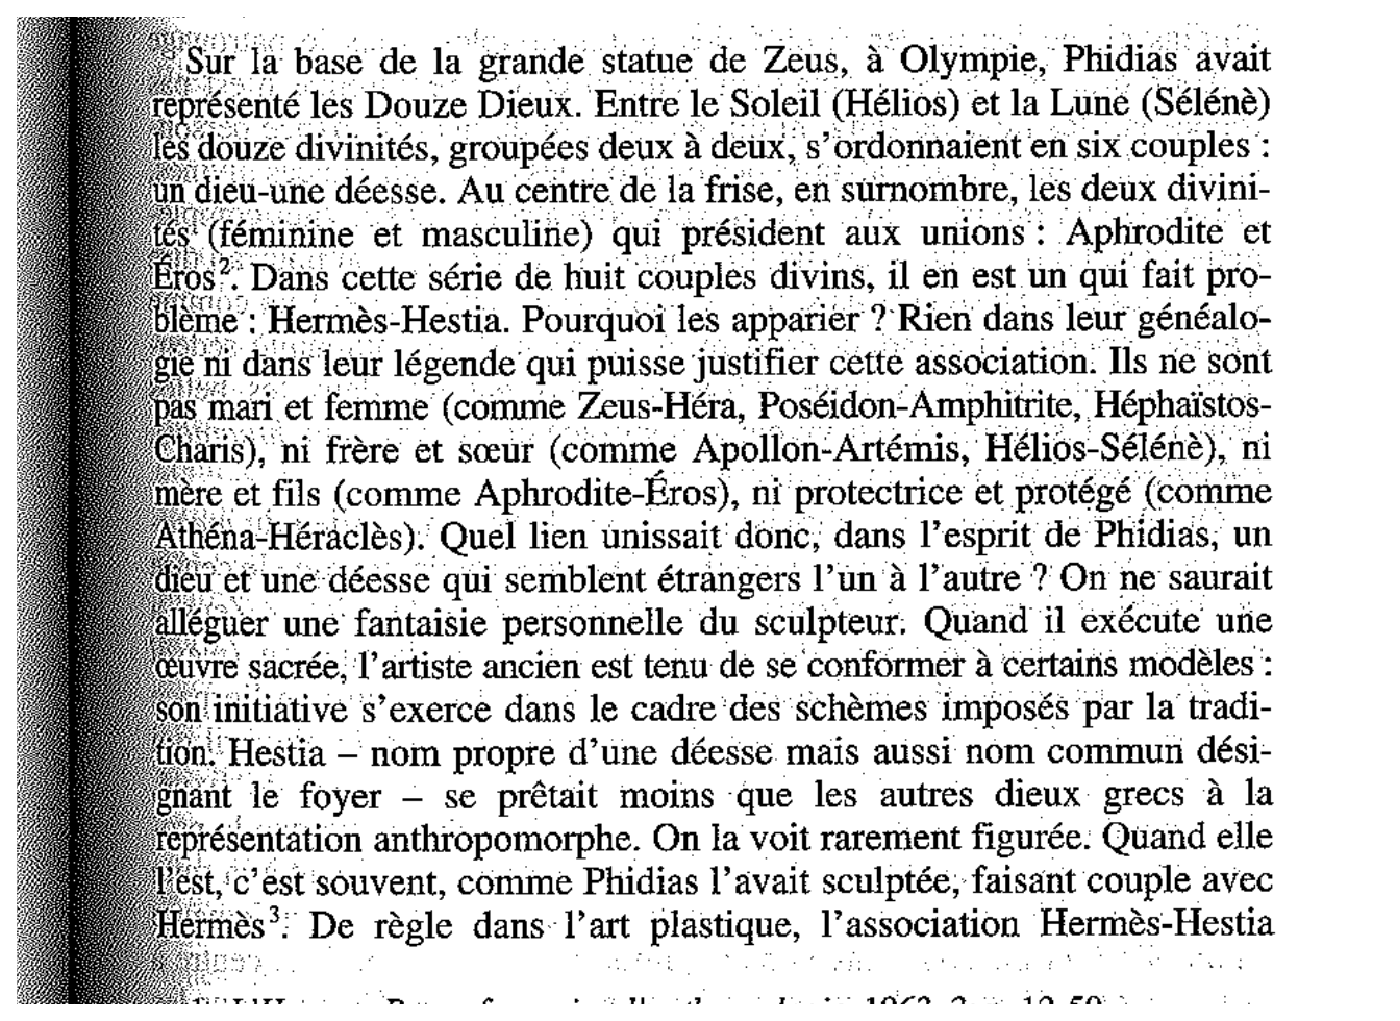
\epsfig{file=figures/despeckling_in.eps,width=0.4\textwidth}}%
      &
      \raisebox{-\height}{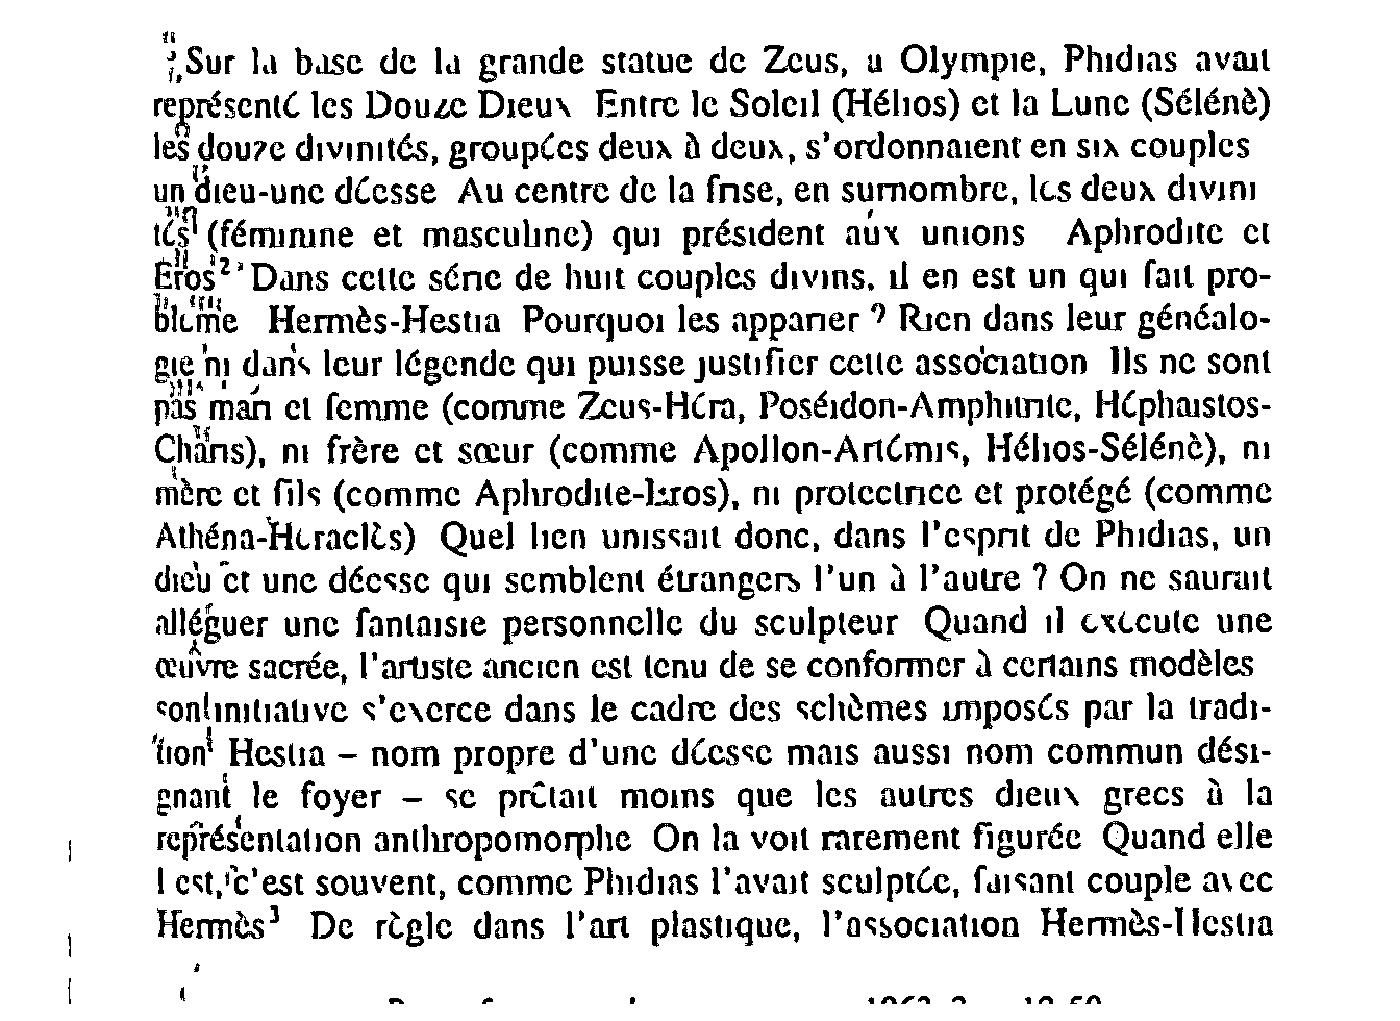
\epsfig{file=figures/despeckling_out.eps,width=0.4\textwidth}}%
    \end{tabular}
  \end{center}
\end{bbawslide}

\begin{bbawslide}{Komponenten eines einfachen OCR-Workflows: Dewarping}
  \vspace*{2mm}%
  \begin{center}
      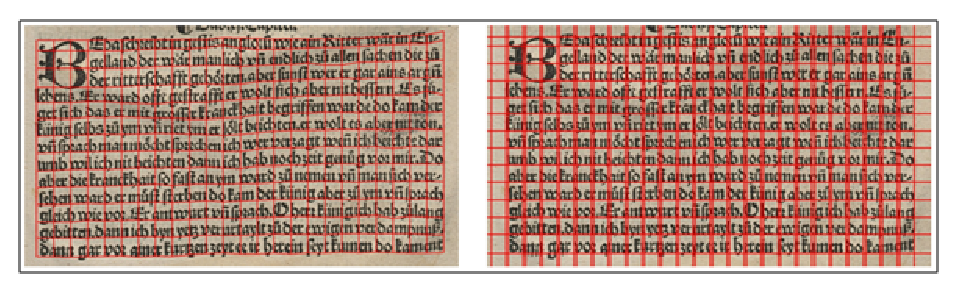
\epsfig{file=figures/dewarping_in_out.eps,width=0.9\textwidth}%
  \end{center}
\end{bbawslide}

\begin{bbawslide}{Komponenten eines OCR-Workflows: Bildvorverarbeitung}
  \vspace*{7mm}%
  \centerslidestrue%
  \textbf{Werkzeuge:}
  \begin{itemize}
    \item Bestandteil der meisten OCR-Programme, häufig jedoch nicht modular
    \item spezielle Tools
    \begin{itemize}\small
      \item \textbf{Scantailor} \url{https://github.com/scantailor/scantailor}
      \begin{description}\footnotesize
        \item[+] umfassendes, frei verfügbares Werkzeug
        \item[-] keine Programmierschnittstelle (API)
      \end{description}
      \item \textbf{Olena/SCRIBO} \url{https://www.lrde.epita.fr/wiki/Olena/Modules#SCRIBO}
      \begin{description}\footnotesize
        \item[+] frei verfügbare Programmierbibliothek für Deskewing, Binarisierung (Implementierung verschiedener Ansätze)
        \item[-] keine Weiterentwicklung/Pflege, schlechtes API-Design
      \end{description}
      \item \textbf{Unpaper} \url{https://github.com/Flameeyes/unpaper}
      \begin{description}\footnotesize
        \item[+] frei verfügbare Programmierbibliothek für Deskewing und Despeckling
      \end{description}
    \end{itemize}
  \end{itemize}
\end{bbawslide}

\begin{bbawslide}{Komponenten eines OCR-Workflows: Bildvorverarbeitung}
  \vspace*{7mm}%
  \centerslidestrue%
  \textbf{Werkzeuge:}
  \begin{itemize}
    \item teilweise auch in Bildbearbeitungsbibliotheken integriert
    \begin{itemize}\small
      \item \textbf{ImageMagick} \url{https://www.imagemagick.org/}
      \begin{description}\footnotesize
        \item[+] extrem umfangreiches, frei verfügbares Softwarepaket
        \item[-] keine spezifische OCR-Implementierung (aber: \url{http://www.fmwconcepts.com/imagemagick/})
      \end{description}
      \item \textbf{Leptonica} \url{http://www.leptonica.com/}
      \begin{description}\footnotesize
        \item[+] sehr umfangreiches, frei verfügbares Softwarepaket
        \item[+] Anwendung in \texttt{Tesseract}
      \end{description}
    \end{itemize}
    \item zahlreiche \textbf{wissenschaftliche Veröffentlichungen} zu einzelnen Aspekten
    \item \textbf{wissenschaftliche Wettbewerbe} zu ausgewählten Aspekten (insb. Binarization und Deskewing)
    \item Forschungsergebnisse finden \textbf{kaum Eingang in die Praxis}
  \end{itemize}
\end{bbawslide}

\begin{bbawslide}{Komponenten eines OCR-Workflows: Layoutanalyse}
  \vspace*{7mm}%
  \centerslidestrue%
  \begin{itemize}
    \item Prozesse zur Erkennung der Struktur auf Seiten- und Dokumentebene
    \begin{itemize}\small
      \item \textbf{Page Segmentation:} Lokalisierung von zusammenhängenden Text- und Nichttextbereichen
      \item \textbf{Region Classification:} Typisierung von Textbereichen
      \item \textbf{Line/Character Splitting:} Lokalisierung der einzelnen Zeilen/Zeichen
      \item \textbf{Document Analysis:} Konstruktion der logischen Dokumentstruktur (METS!)
    \end{itemize}
    \item entscheidend für die korrekte \textbf{Rekonstruktion des Textflusses} und damit für maschinelle Auswertungen
  \end{itemize}
\end{bbawslide}

\begin{bbawslide}{Komponenten eines OCR-Workflows: Layoutanalyse}
  \vspace*{2mm}%
  \centerslidesfalse%
  \begin{tabular}{cc}
    \raisebox{-\height}{\parbox{7cm}{%
      \begin{itemize}
        \item \textbf{strukturierende} Elemente
        \begin{itemize}
          \item Absätze
          \item Überschriften
        \end{itemize}
      \end{itemize}
    }}
    &
    \raisebox{-\height}{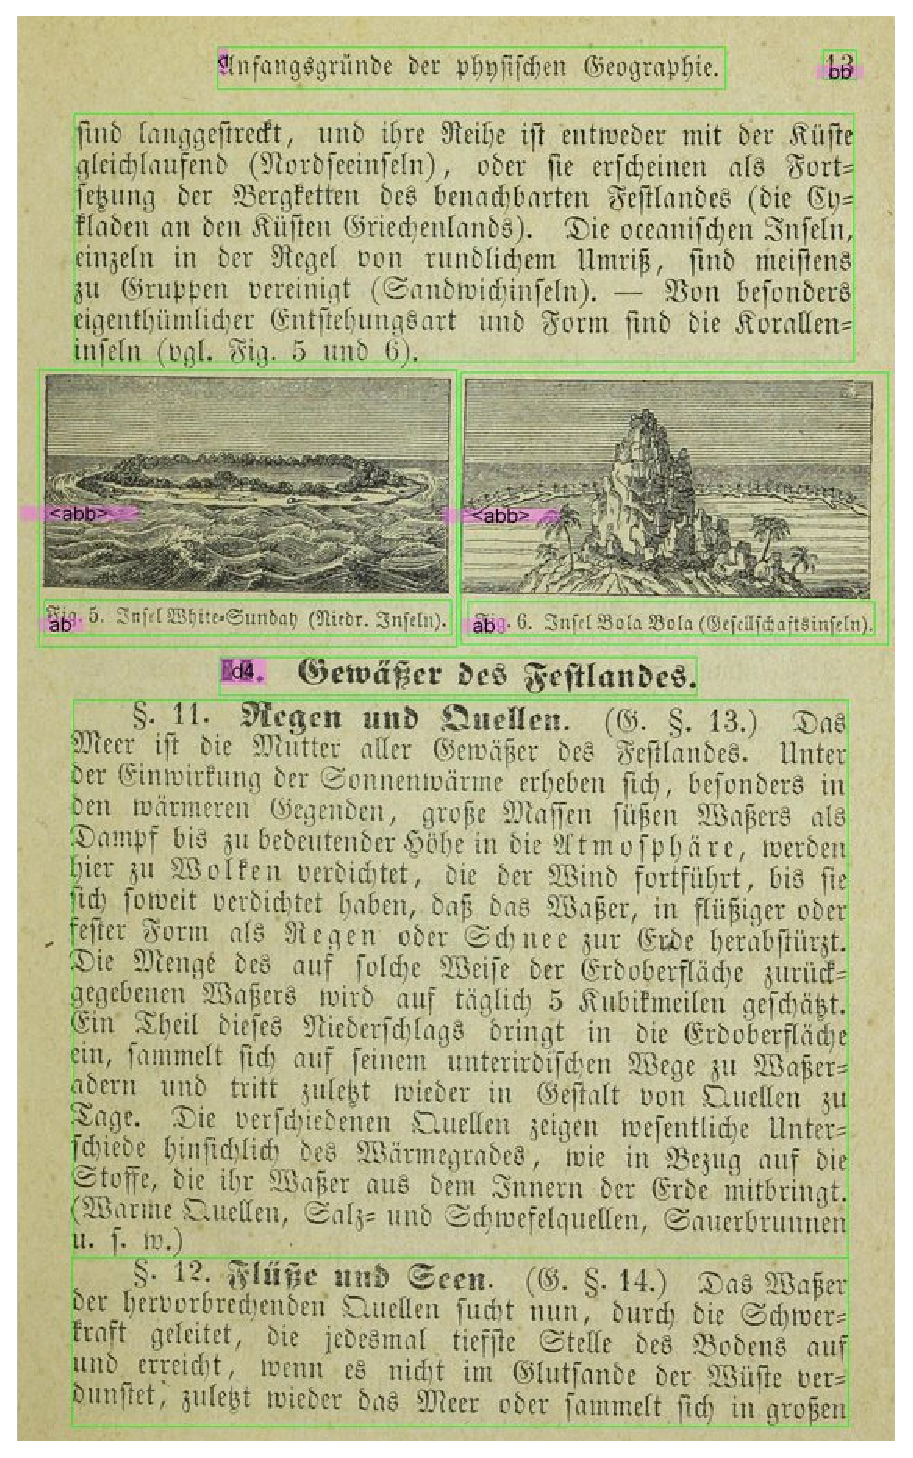
\epsfig{file=figures/layout_rec_example.eps,width=0.4\textwidth}}%
  \end{tabular}
\end{bbawslide}

\begin{bbawslide}{Komponenten eines OCR-Workflows: Layoutanalyse}
  \vspace*{2mm}%
  \centerslidesfalse%
  \begin{tabular}{cc}
    \raisebox{-\height}{\parbox{7cm}{%
      \begin{itemize}
        \item \textbf{strukturierende} Elemente
        \begin{itemize}
          \item Absätze
          \item Überschriften
        \end{itemize}
        \item \textbf{textflussunterbrechende} Elemente
        \begin{itemize}
          \item Seitenzahlen
          \item Kolumnentitel
          \item Abbildungsunterschriften
          \item Marginalien etc.
        \end{itemize}
      \end{itemize}
    }}
    &
    \raisebox{-\height}{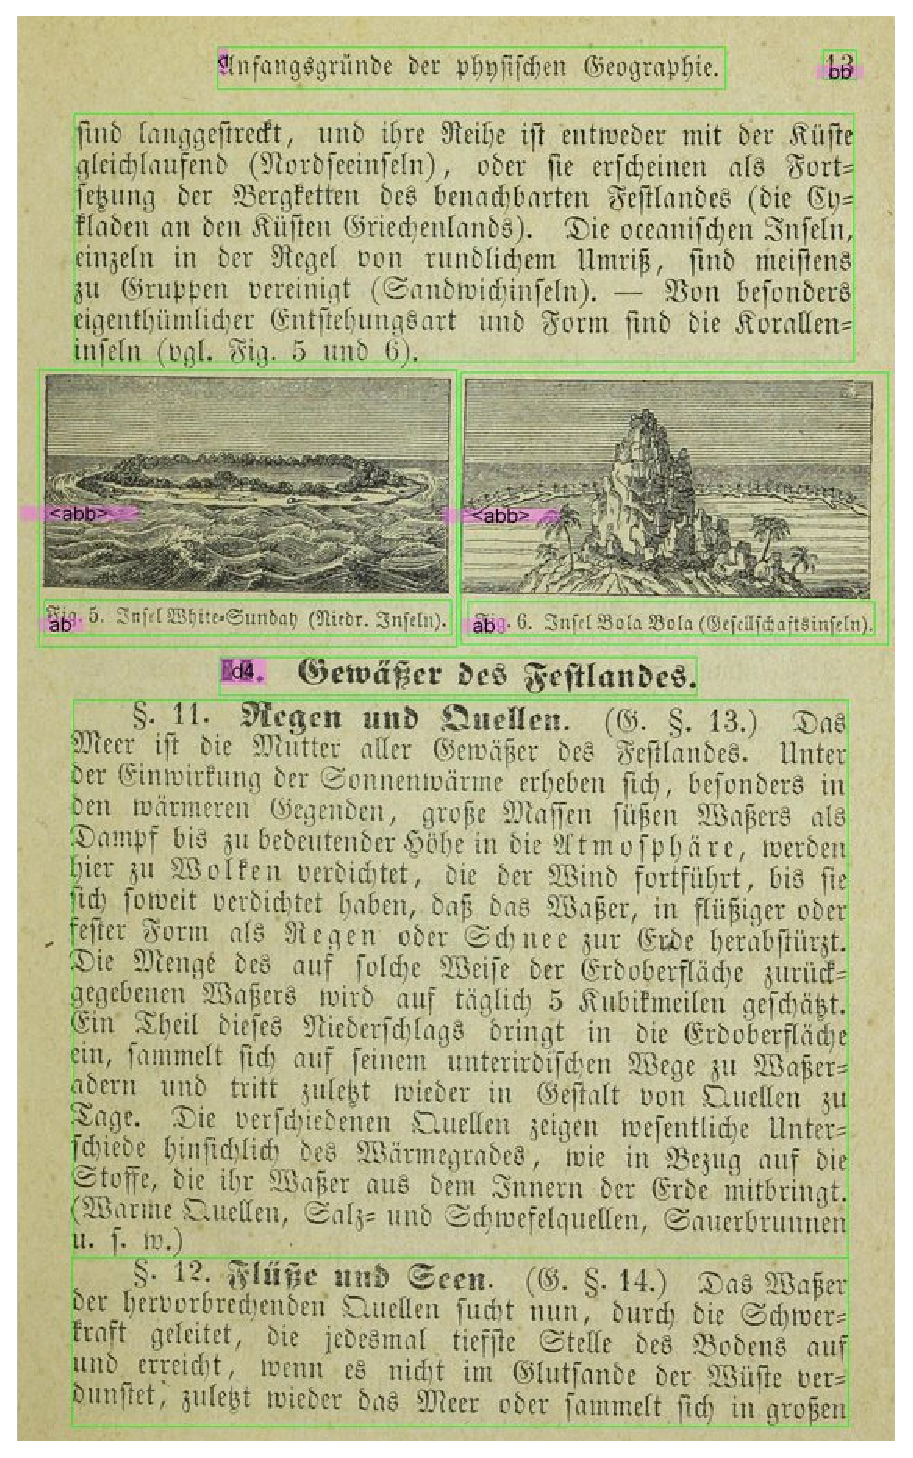
\epsfig{file=figures/layout_rec_example.eps,width=0.4\textwidth}}%
  \end{tabular}
\end{bbawslide}

\begin{bbawslide}{Komponenten eines OCR-Workflows: Layoutanalyse}
  \vspace*{2mm}%
  \centerslidesfalse%
  \begin{tabular}{cc}
    \raisebox{-\height}{\parbox{7cm}{%
      \begin{itemize}
        \item \textbf{strukturierende} Elemente
        \begin{itemize}
          \item Absätze
          \item Überschriften
        \end{itemize}
        \item \textbf{textflussunterbrechende} Elemente
        \begin{itemize}
          \item Seitenzahlen
          \item Kolumnentitel
          \item Abbildungsunterschriften
          \item Marginalien etc.
        \end{itemize}
        \item \textbf{nichttextuelle} Elemente
        \begin{itemize}
          \item Abbildungen
          \item Tabellen
        \end{itemize}
      \end{itemize}
    }}
    &
    \raisebox{-\height}{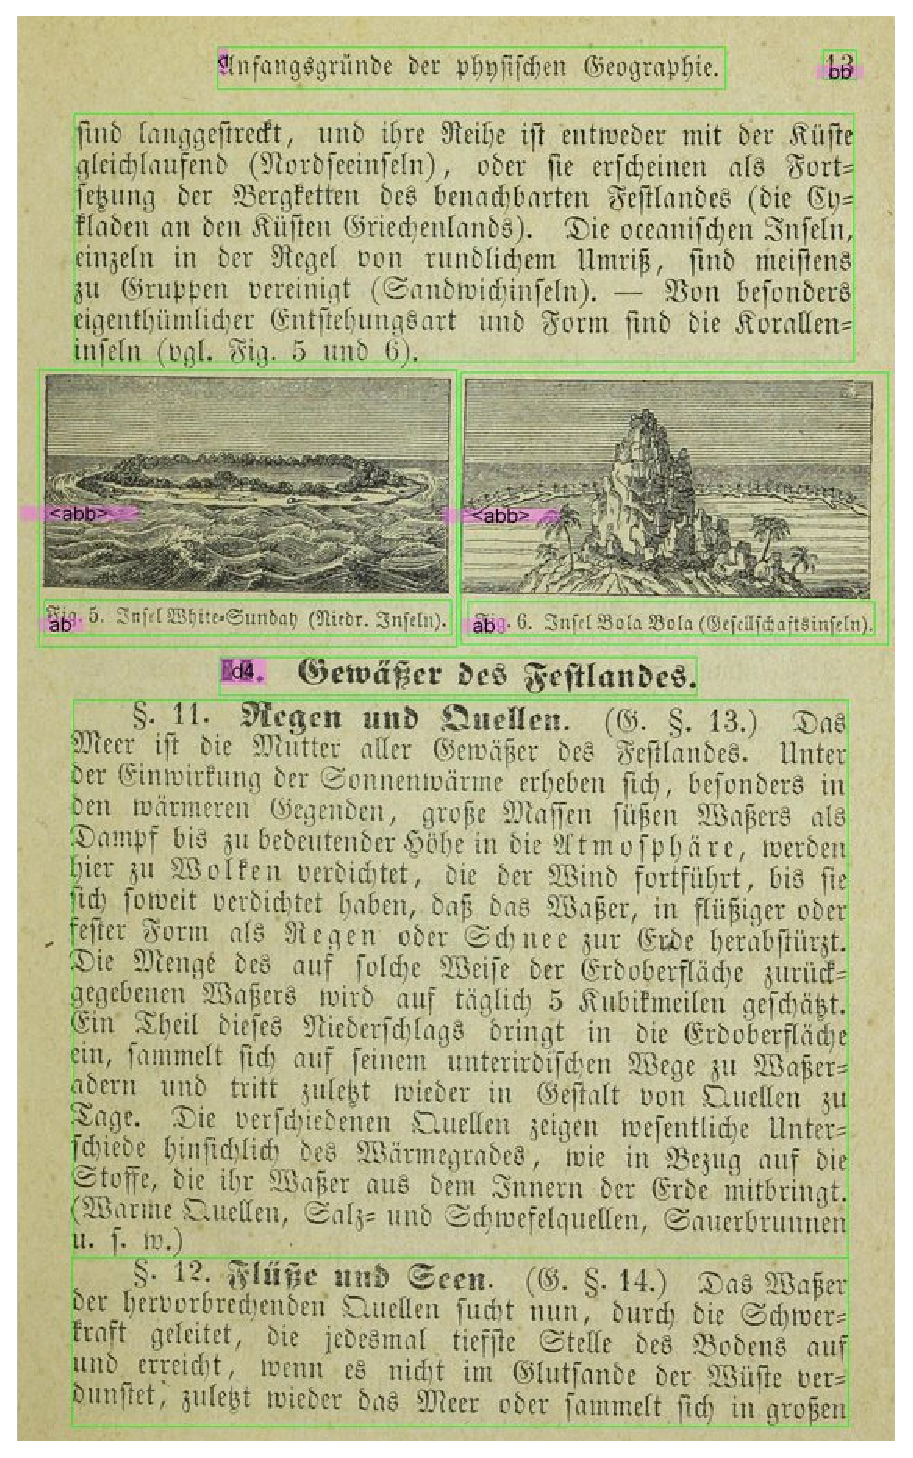
\epsfig{file=figures/layout_rec_example.eps,width=0.4\textwidth}}%
  \end{tabular}
\end{bbawslide}

\begin{bbawslide}{Komponenten eines OCR-Workflows: Layoutanalyse}
  \vspace*{2mm}%
  \centerslidestrue%
  \textbf{Werkzeuge:}
  \begin{itemize}
    \item auch bei der OLR \textbf{Missverhältnis} zwischen Forschungsergebnissen und verfügbaren Lösungen
    \item OCR-Programme implementieren einfache Lösungen zur Page Segmentation, teilweise separat adressierbar
    \begin{itemize} \small
        \item Klassifizierung beschränkt sich im Wesentlichen auf Text vs. Nichttext
        \item Qualität auf schwierigen Vorlagen überschaubar
    \end{itemize}
    \item wissenschaftliche Wettbewerbe und Untersuchungen befassen sich mit der Erkennung \textbf{komplexer Layouts} und \textbf{Dokumentstukturierung}
    \item jedoch \textbf{keine umfassenden} Ansätzen (Kustoden, Marginalien, Bogensignaturen)
    \item ebenfalls kaum Forschung zu \textbf{polygonen Zonen}
  \end{itemize}
\end{bbawslide}

\begin{bbawslide}{Komponenten eines OCR-Workflows: Layoutanalyse}
  \vspace*{2mm}%
  \centerslidestrue%
  \textbf{Werkzeuge:}
  \begin{itemize}
    \item einzelner Befehl für Seiten- und Zeilensegmentierung in \texttt{OCRopus} 
    \begin{itemize}\small
      \item im Ergebnis nur Einzelbilder auf Zeilenebene
      \item \textbf{keine Koordinaten}, kein Zugriff auf Seitensegmentierung
    \end{itemize}
    \item Zugriff auf alle Ebenen der Seitensegmentierung in \texttt{Tesseract}
    \begin{itemize}\small
      \item \textbf{inklusive Koordinaten}
      \item basale Klassifizierung der Segmente (Spalten, Abbildungen, Formeln, Tabellen, Text)
    \end{itemize}
    \item Layouterkennungswerkzeug \texttt{Larex} \hlcite{Reul at al. 2017}
    \begin{itemize}\small
      \item Festlegung buchspezifischer Parameter durch den Nutzer (Spalten, Kolumnentitel etc.) für Klassifizierungsaufgabe
      \item manuelle Nachkorrektur über Benutzeroberfläche
      \item inklusive Zeilenerkennung, open-source: \url{https://github.com/chreul/LAREX}, keine API
    \end{itemize}
  \end{itemize}
\end{bbawslide}

\begin{bbawslide}{Komponenten eines OCR-Workflows: Texterkennung}
  \vspace*{7mm}%
  \centerslidestrue%
  \begin{itemize}
    \item Kernkomponente der OCR
    \item Genauigkeit beeinflusst vom Typ des zugrundeliegenden \textbf{Algorithmus} und vom eingesetzten \textbf{Modell}
    \item aktuell Paradigmenwechsel: \textbf{zeichenorientiert} $\rightarrow$ \textbf{zeilenorientiert}
    \begin{itemize} \small
      \item \textbf{Deep learning:} Tiefe (i.e.~vielschichtige) neuronale Netzwerke zur Sequenzklassifizierung \hlcite{Hochreiter und Schmidhuber 1997}
      \item wesentlich weniger anfällig für \textbf{Zeichenvarianz}
      \item eingebautes \textbf{Sprachmodell}
    \end{itemize}
    \item auch schwierige historische Vorlagen in \enquote{OCR-Reichweite} \hlcite{Springmann 2016}
  \end{itemize}
\end{bbawslide}

\begin{bbawslide}{Komponenten eines OCR-Workflows: Texterkennung}
  \vspace*{7mm}%
  \centerslidestrue%
  \textbf{Werkzeuge:}
  \begin{itemize}
    \item überraschend viele verfügbare OCR-Engines
    \item \url{https://github.com/kba/awesome-ocr}
    \item Abbyy \texttt{FineReader} am verbreitetsten im produktiven Einsatz
    \item zwei Platzhirsche im \textbf{Open-Source-Bereich}
    \item \texttt{Tesseract} \url{https://github.com/tesseract-ocr/tesseract}
    \begin{itemize}\small
      \item ursprünglich von Hewlett-Packard entwickelt
      \item von Google übernommen und Open-Source gestellt
      \item viele \textbf{mitgelieferte Modelle} (auch für Fraktur)
      \item mit Version 4 Umstieg auf zeilenorientiert Erkennung auf Basis neuronaler Netze
    \end{itemize}
  \end{itemize}
\end{bbawslide}

\begin{bbawslide}{Komponenten eines OCR-Workflows: Texterkennung}
  \vspace*{7mm}%
  \centerslidestrue%
  \textbf{Werkzeuge:}
  \begin{itemize}
    \item \texttt{OCRopus} \url{https://github.com/tmbdev/ocropy}
    \begin{itemize}\small
      \item entwickelt von Thomas Breul mit Unterstützung von Google
      \item ursprünglich als Wrapper für Tesseract, später mit eigener Erkennungsroutine auf Basis neuronaler Netze
      \item nur wenige \textbf{mitgelieferte Modelle}
    \end{itemize}
    \item \texttt{Gamera} \url{https://github.com/hsnr-gamera/gamera}
    \begin{itemize}\small
      \item komplettes Framework für Layoutanalyse und Texterkennung
      \item zeichenorientierter Ansatz auf Basis des \enquote{$k$ nearest neighbor}-Algorithmus'
      \item nur ein \textbf{mitgeliefertes Modell}
    \end{itemize}
  \end{itemize}
\end{bbawslide}

\begin{bbawpart}{\Large\bf Modelltraining}
\end{bbawpart}

\begin{bbawslide}{Modelltraining}
  \vspace*{7mm}%
  \centerslidestrue%
  \begin{itemize}
    \item Texterkennung auf Basis \textbf{statistischer} Modelle
    \begin{itemize}\small
      \item Induktion anhand manuell erstellter Trainingsdaten (i.e.~\textbf{Ground Truth})
      \item Wahrscheinlichkeitsverteilung abhängig vom Modelltyp entweder direkt berechnet oder (iterativ) optimiert
    \end{itemize}
    \item unterschiedliche Ansätze erfordern unterschiedliche \textbf{Trainingsprozeduren}
    \item grundsätzliches Vorgehen jedoch gleich $\rightarrow$ \textbf{Alignierung} von Text und Bild
    \begin{itemize}\small
      \item unterschiedliche Anforderung an \textbf{Annotationstiefe}
      \item Qualität und Quantität der Trainingsdaten bestimmt Qualität der Modelle
    
    \end{itemize}
    \item Kompromiss zwischen \textbf{Übertragbarkeit} und spezifischer Textqualität
    \begin{itemize}\small
      \item mitgelieferte Modelle häufig zu \enquote{allgemein}
      \item Qualität der Texterkennung im Vergleich zu Standardmodellen \textbf{signifikant höher} \hlcite{Springmann et al. 2015}
    \end{itemize}
  \end{itemize}
\end{bbawslide}

\renewcommand{\footerText}{\tiny 4. August 2017, DH-Kolloquium, BBAW\hspace{4cm} Image by Uwe Springmann, CC BY-SA 4.0}

\begin{bbawslide}{Modelltraining: Trainingsdaten}
  \vspace*{2mm}%
  \centerslidestrue%
  \begin{tabular}{cc}
    \raisebox{-\height}{\parbox{7cm}{%
    \begin{itemize}
      \item Digitalisate und zugehöriger, \textbf{fehlerfreier} Volltext
      \item Alignierung auf Zeichen- oder Zeilenebene
      \item \textbf{zeichenorientierte} Ansätze: jedes Zeichen mindestens einmal im Trainingsmaterial
      \item \textbf{zeilenorientierte} Ansätze: ca. 10 Seiten eines Buches
      \item \texttt{Tesseracts} \enquote{Latin model} (i.e. großmaßstäbliches Mehrsprachenmodell für Antiquaschriftarten): ca. \numprint{400000} Zeilen in ca. \numprint{4500} Schriftarten
    \end{itemize}
    }}
    &
    \raisebox{-\height}{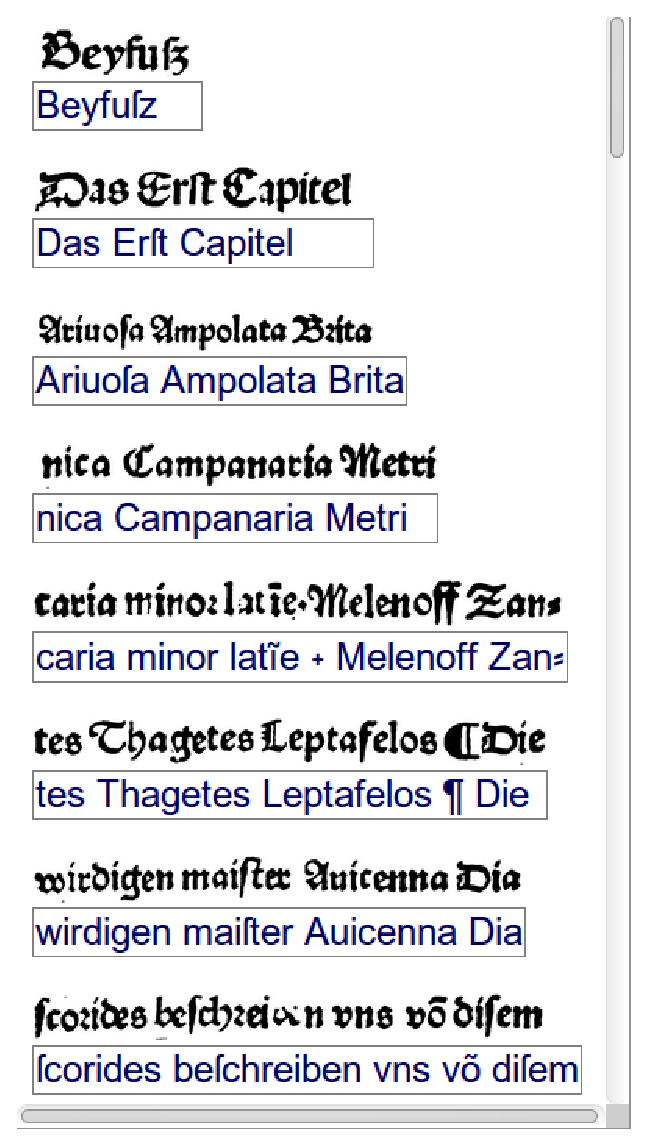
\epsfig{file=figures/gt.eps,width=0.3\textwidth}}%
  \end{tabular}
\end{bbawslide}

\renewcommand{\footerText}{\tiny 4. August 2017, DH-Kolloquium, BBAW}

\begin{bbawslide}{Modelltraining: Trainingseffekte}
  \vspace*{2mm}%
  \centerslidestrue%
  \begin{center}
    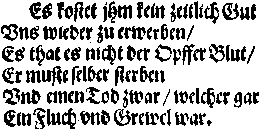
\epsfig{file=figures/train.eps,width=0.4\textwidth}\\
    \begin{tabular}{l@{\hspace{2cm}}l}
      Abbyy \texttt{Finereader 11} & \texttt{OCRopus} \\
      \begin{minipage}{0.4\textwidth}
        ES kostet Om kein zeitlich Gut  
        Dns wieder zu erwerben/\\
        ES that es nicht der OpfferBluk/\\
        Cr muste selber sterben\\
        Vnd emenTod zwar/ welcher gar\\
        EinFluch vnd Grcwcl war.
      \end{minipage}
      & 
      \begin{minipage}{0.4\textwidth}
        Es kostet jzm kein zattlchGut\\
        Bns wteder zu crwerben?\\
        Es that cs mcht der OpfferBlut?  
        Ermustcselbcr stcrbcn\\
        Bnd emnenTodzwar, welchae gar\\
        EtFluchvnd Grcwewar.
      \end{minipage}
    \end{tabular}
  \end{center}
\end{bbawslide}

\begin{bbawslide}{Modelltraining: Trainingseffekte}
  \vspace*{2mm}%
  \centerslidestrue%
  \begin{center}
    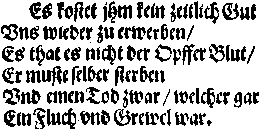
\epsfig{file=figures/train.eps,width=0.4\textwidth}\\
    \begin{tabular}{l@{\hspace{2cm}}l}
      Abbyy \texttt{Finereader 11} & \texttt{OCRopus} (homebrew)\\
      \begin{minipage}{0.4\textwidth}
        ES kostet Om kein zeitlich Gut  
        Dns wieder zu erwerben/\\
        ES that es nicht der OpfferBluk/\\
        Cr muste selber sterben\\
        Vnd emenTod zwar/ welcher gar\\
        EinFluch vnd Grcwcl war.
      \end{minipage}
      & 
      \begin{minipage}{0.4\textwidth}
        Es ko\textlongs\textbf{\textcolor{red}{l}}et jhm kein zeitlich Gut  
        Vns wieder zu \textbf{\textcolor{red}{t}}erwerben/  
        Es that es nicht der Opffer Blut/  
        Er mu\textlongs{}te \textlongs{}elber \textlongs{}terben  
        Vnd einen Tod zwar/ welcher gar  
        Ein Fluch vnd Grewel war.
      \end{minipage}
    \end{tabular}
  \end{center}
\end{bbawslide}

\begin{bbawslide}{Modelltraining: Werkzeuge}
  \vspace*{7mm}%
  \centerslidestrue%
  \begin{itemize}
    \item jede OCR-Software kommt mit \textbf{eigener Trainingsprozedur}
    \item zahlreiche \enquote{ease-of-use}-Wrapper:
    \begin{itemize}
      \item \texttt{Tesseract}: \texttt{VietOCR}, \texttt{Aletheia}, \texttt{Franken++}
      \item \texttt{OCRopus}: \texttt{OCRocis}, HTML-Wrapper
    \end{itemize}
    \item Probleme:
    \begin{itemize}
      \item teilweise \textbf{kostenpflichtig} (\texttt{Aletheia}) bzw. nicht mehr gepflegt (\texttt{Franken++})
      \item teilweise zu \textbf{umständlich} in der Bedienung (\texttt{OCRopus}-Training, \texttt{Aletheia})
    \end{itemize}
\end{itemize}
\end{bbawslide}

\begin{bbawpart}{\Large\bf Optimierungsoptionen}
\end{bbawpart}

\begin{bbawslide}{Optimierungsoptionen: Lokale Bildoptimierung}
  \vspace*{7mm}%
  \centerslidestrue%
  \begin{itemize}
    \item historische Vorlagen bzw. ältere Digitalisate oftmals suboptimal für OCR
    \begin{itemize}\small
      \item unterschiedliche \textbf{Beleuchtung}
      \item charakteristische \textbf{Trapezform}
    \end{itemize}
    \item verschiedene Bearbeitungsebenen
    \begin{itemize}\small
      \item Dokument, Seite, Absatz (bzw. Textzone), Zeile
      \item Operationen greifen \textbf{wiederholt} auf verschiedenen Ebenen ein
      \item \textbf{maximale Adaptivität} bzgl. spezifischer Charakteristika auf Bild- und Textebene
      \item Rekonstruierbarkeit über Metadaten (z.B.~Koordinaten) zu gewährleisten
    \end{itemize}
  \end{itemize}
\end{bbawslide}

\begin{bbawslide}{Optimierungsoptionen: Lokale Bildoptimierung}
  \vspace*{2mm}%
  \centerslidestrue%
  \begin{tabular}{cc}
    \raisebox{-\height}{\parbox{7cm}{%
    \textbf{Rezept:}
    \begin{enumerate}
      \item \textbf{Bildoptimierung} auf Seitenebene
      \item \textbf{Seitensegmentierung} auf Seitenebene
      \item \textbf{Extraktion} der Segmente aus dem (nichtoptimierten) Original
      \item \textbf{Bildoptimierung} auf Segmentebene
      \item \textbf{Zeilensegmentierung} auf Segmentebene
      \item \textbf{Extraktion} der Zeile aus dem (nichtoptimierten) Segment
      \item \textbf{Bildoptimierung} auf Zeilenebene
    \end{enumerate}
    }}
    &
    \raisebox{-\height}{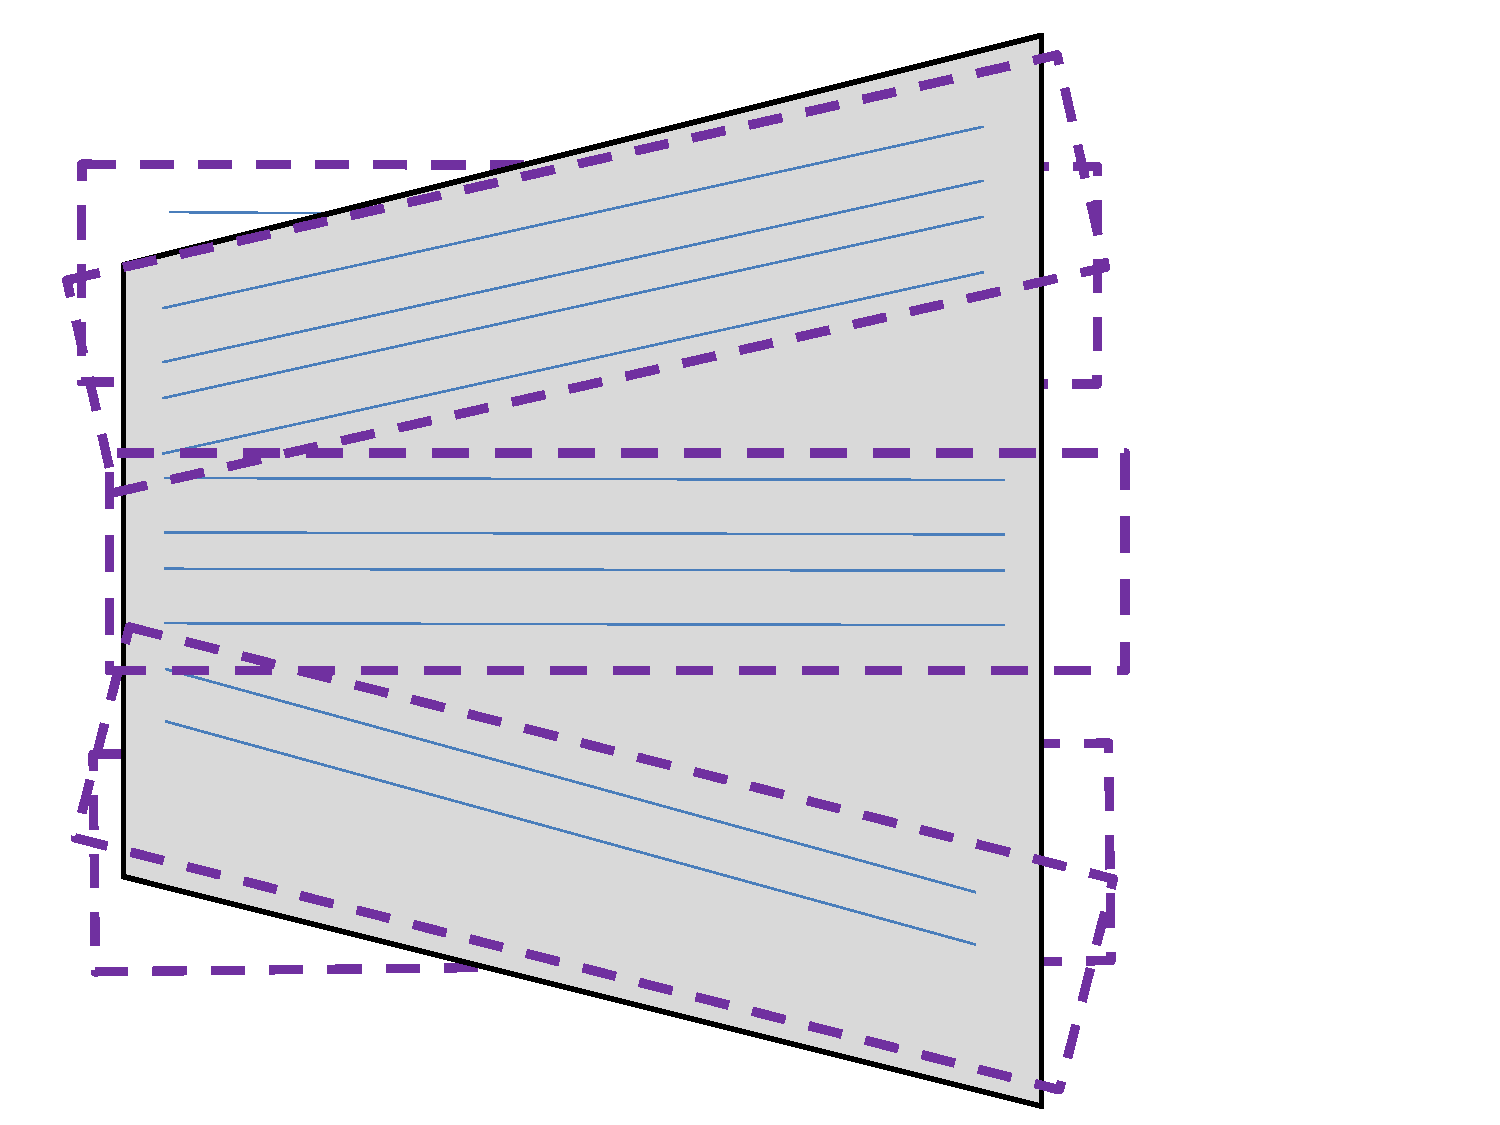
\epsfig{file=figures/deskewing_ex2.eps,width=0.5\textwidth}}%
  \end{tabular}
\end{bbawslide}

\begin{bbawslide}{Optimierungsoptionen: OCR-Merging}
  \vspace*{7mm}%
  \centerslidestrue%
  \begin{itemize}
    \item Prozesse zur \textbf{Vereinigung} verschiedener OCR-Ergebnisse \textbf{in einen Volltext}
    \item Fehler auch bei \enquote{optimaler} Vorverarbeitung und Verwendung spezifischer Modelle
    \item \textbf{unterschiedliche Engines} bzw. Modelle haben \textbf{unterschiedliche Stärken} und machen unterschiedliche Fehler
    \item Idee: \textbf{Extraktion} korrekt erkannter Textbestandteile \textbf{aus mehreren OCR-Durchgängen} \hlcite{Handley 1998}
    \item Vorteil: Integration vorhandener OCR ebenfalls möglich
    \item \textbf{Reduktion} der Anzahl der falsch erkannten Zeichen\\um 14~\% erzielt \hlcite{Boenig et al. 2016} 
  \end{itemize}
\end{bbawslide}

\begin{bbawslide}{OCR-Merging: Kotzebue \enquote{Schutzgeist} (1814)}
    \begin{tabular}{cc}
    & \texttt{Abbyy Finereader}\\
      \begin{minipage}{0.5\textwidth}
        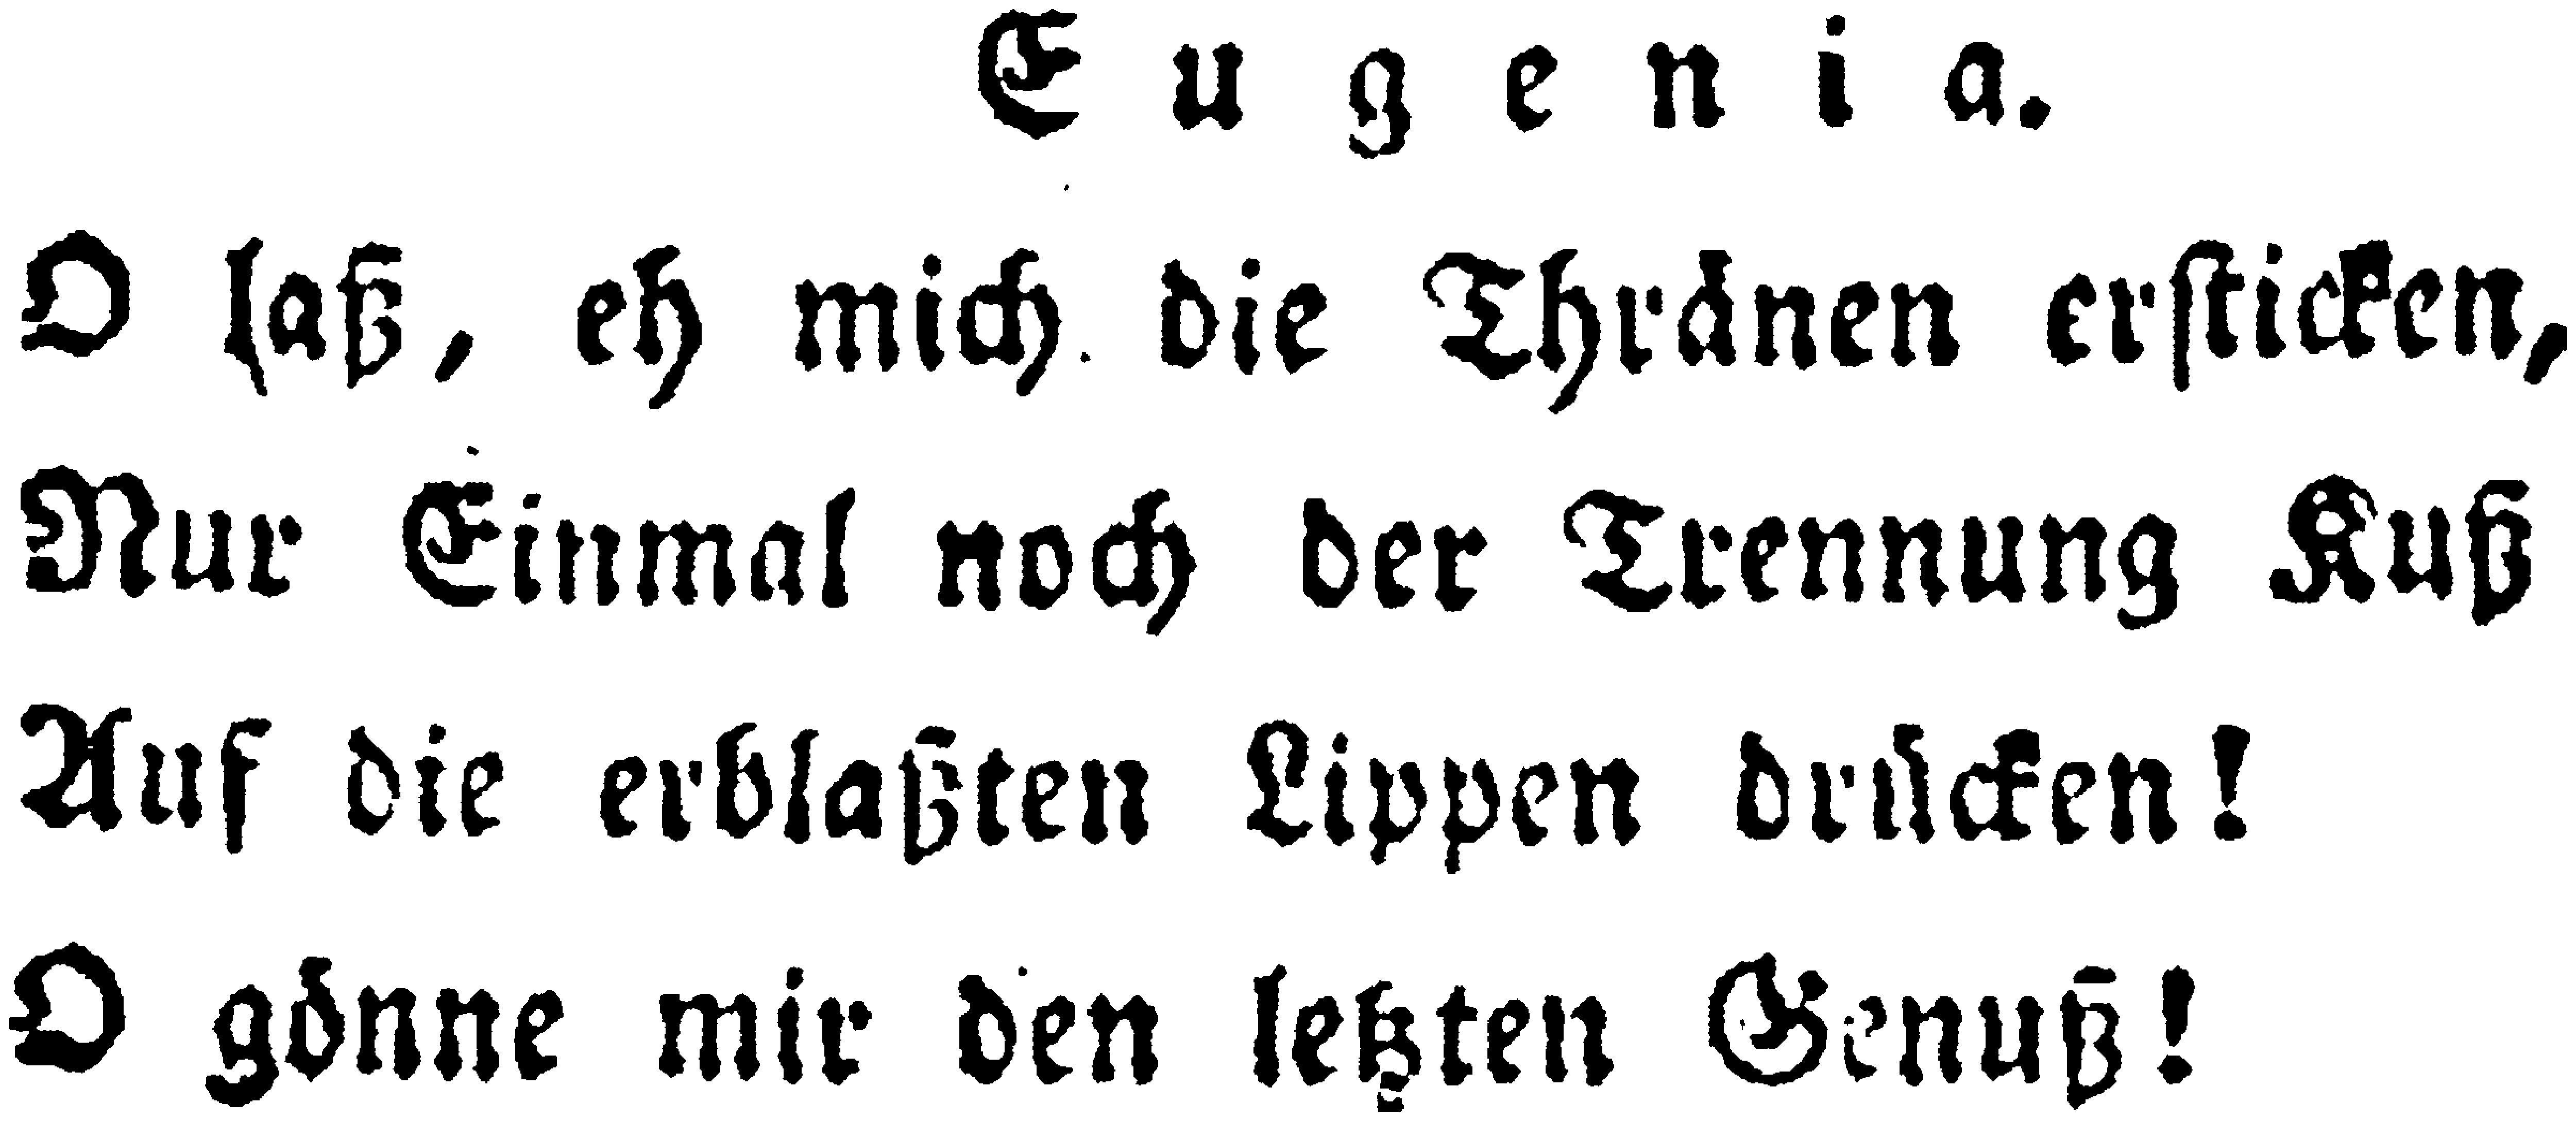
\epsfig{file=figures/example1.eps,width=\textwidth}
      \end{minipage}
      &
      \begin{minipage}{0.5\textwidth}
        E u g e n i a.\\
        O \textbf{\textcolor{bbawred}{§}}aß, eh mich die Thränen ersticken.\\
        Nur Einmal noch der Trennung Kuß\\
        Auf die erblaßten Lippen drücken!\\
        O gönne mir den le\textbf{\textcolor{bbawred}{h}}ten Genuß!
      \end{minipage}\\\\
      \phantom{\texttt{Tesseract}} & \phantom{\texttt{OCRopus}}\\
      \phantom{
      \begin{minipage}{0.5\textwidth}
        Eugeaia.\\
        O laß, H) mich. die Tht*äaea erIHckm,\\
        Nur Einqu noch der Trennung Kuß\\
        Auf die erqußteu Lippen drückenx\\
        O gönne mie den legten Genußx
      \end{minipage}}
      &
      \phantom{
      \begin{minipage}{0.5\textwidth}
        E u g e n i a.\\
        O \textbf{\textcolor{bbawred}{h}}aß, eh mich die Thränen ersticken,\\
        Nur Einmal noch der Trennung Kuß\\
        Auf die erblaßten Lippen drücken!\\
        O g\textbf{\textcolor{bbawred}{d}}nne mir den letzten Genuß!
      \end{minipage}
      }
    \end{tabular}
    \vspace{-2em}
\end{bbawslide}

\begin{bbawslide}{OCR-Merging: Kotzebue \enquote{Schutzgeist} (1814)}
    \begin{tabular}{cc}
    & \texttt{Abbyy Finereader}\\
      \begin{minipage}{0.5\textwidth}
        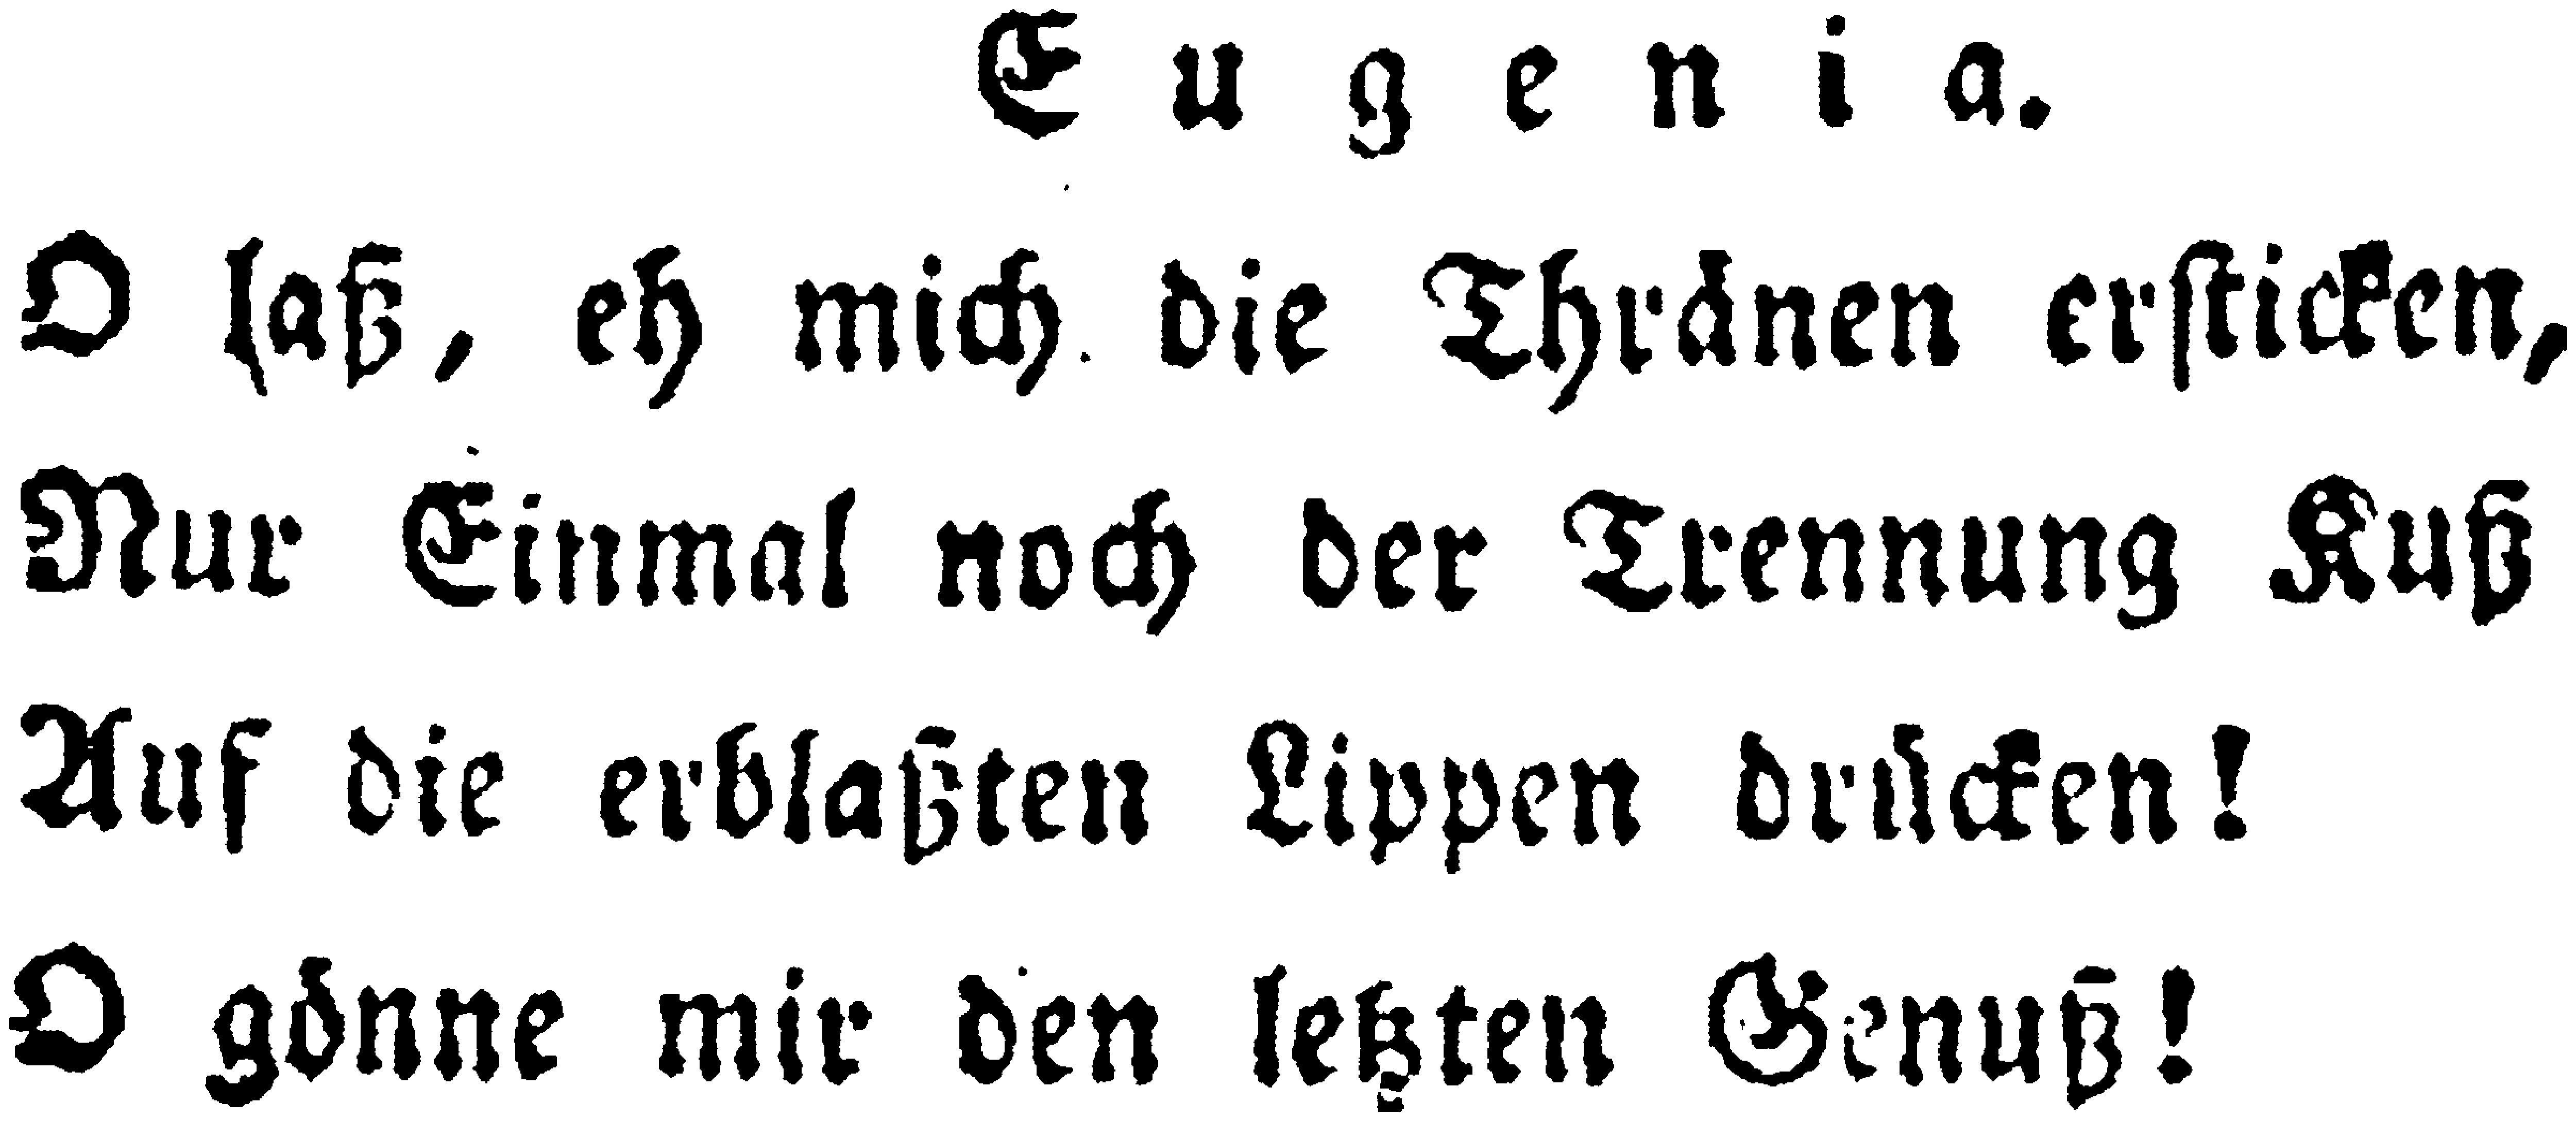
\epsfig{file=figures/example1.eps,width=\textwidth}
      \end{minipage}
      &
      \begin{minipage}{0.5\textwidth}
        E u g e n i a.\\
        O \textbf{\textcolor{bbawred}{§}}aß, eh mich die Thränen ersticken.\\
        Nur Einmal noch der Trennung Kuß\\
        Auf die erblaßten Lippen drücken!\\
        O gönne mir den le\textbf{\textcolor{bbawred}{h}}ten Genuß!
      \end{minipage}\\\\
      \texttt{Tesseract} & \phantom{\texttt{OCRopus}}\\
      \begin{minipage}{0.5\textwidth}
        Eugeaia.\\
        O laß, H) mich. die Tht*äaea erIHckm,\\
        Nur Einqu noch der Trennung Kuß\\
        Auf die erqußteu Lippen drückenx\\
        O gönne mie den legten Genußx
      \end{minipage}
      &
      \phantom{
      \begin{minipage}{0.5\textwidth}
        E u g e n i a.\\
        O \textbf{\textcolor{bbawred}{h}}aß, eh mich die Thränen ersticken,\\
        Nur Einmal noch der Trennung Kuß\\
        Auf die erblaßten Lippen drücken!\\
        O g\textbf{\textcolor{bbawred}{d}}nne mir den letzten Genuß!
      \end{minipage}
      }
    \end{tabular}
    \vspace{-2em}
\end{bbawslide}

\begin{bbawslide}{OCR-Merging: Kotzebue \enquote{Schutzgeist} (1814)}
    \begin{tabular}{cc}
    & \texttt{Abbyy Finereader}\\
      \begin{minipage}{0.5\textwidth}
        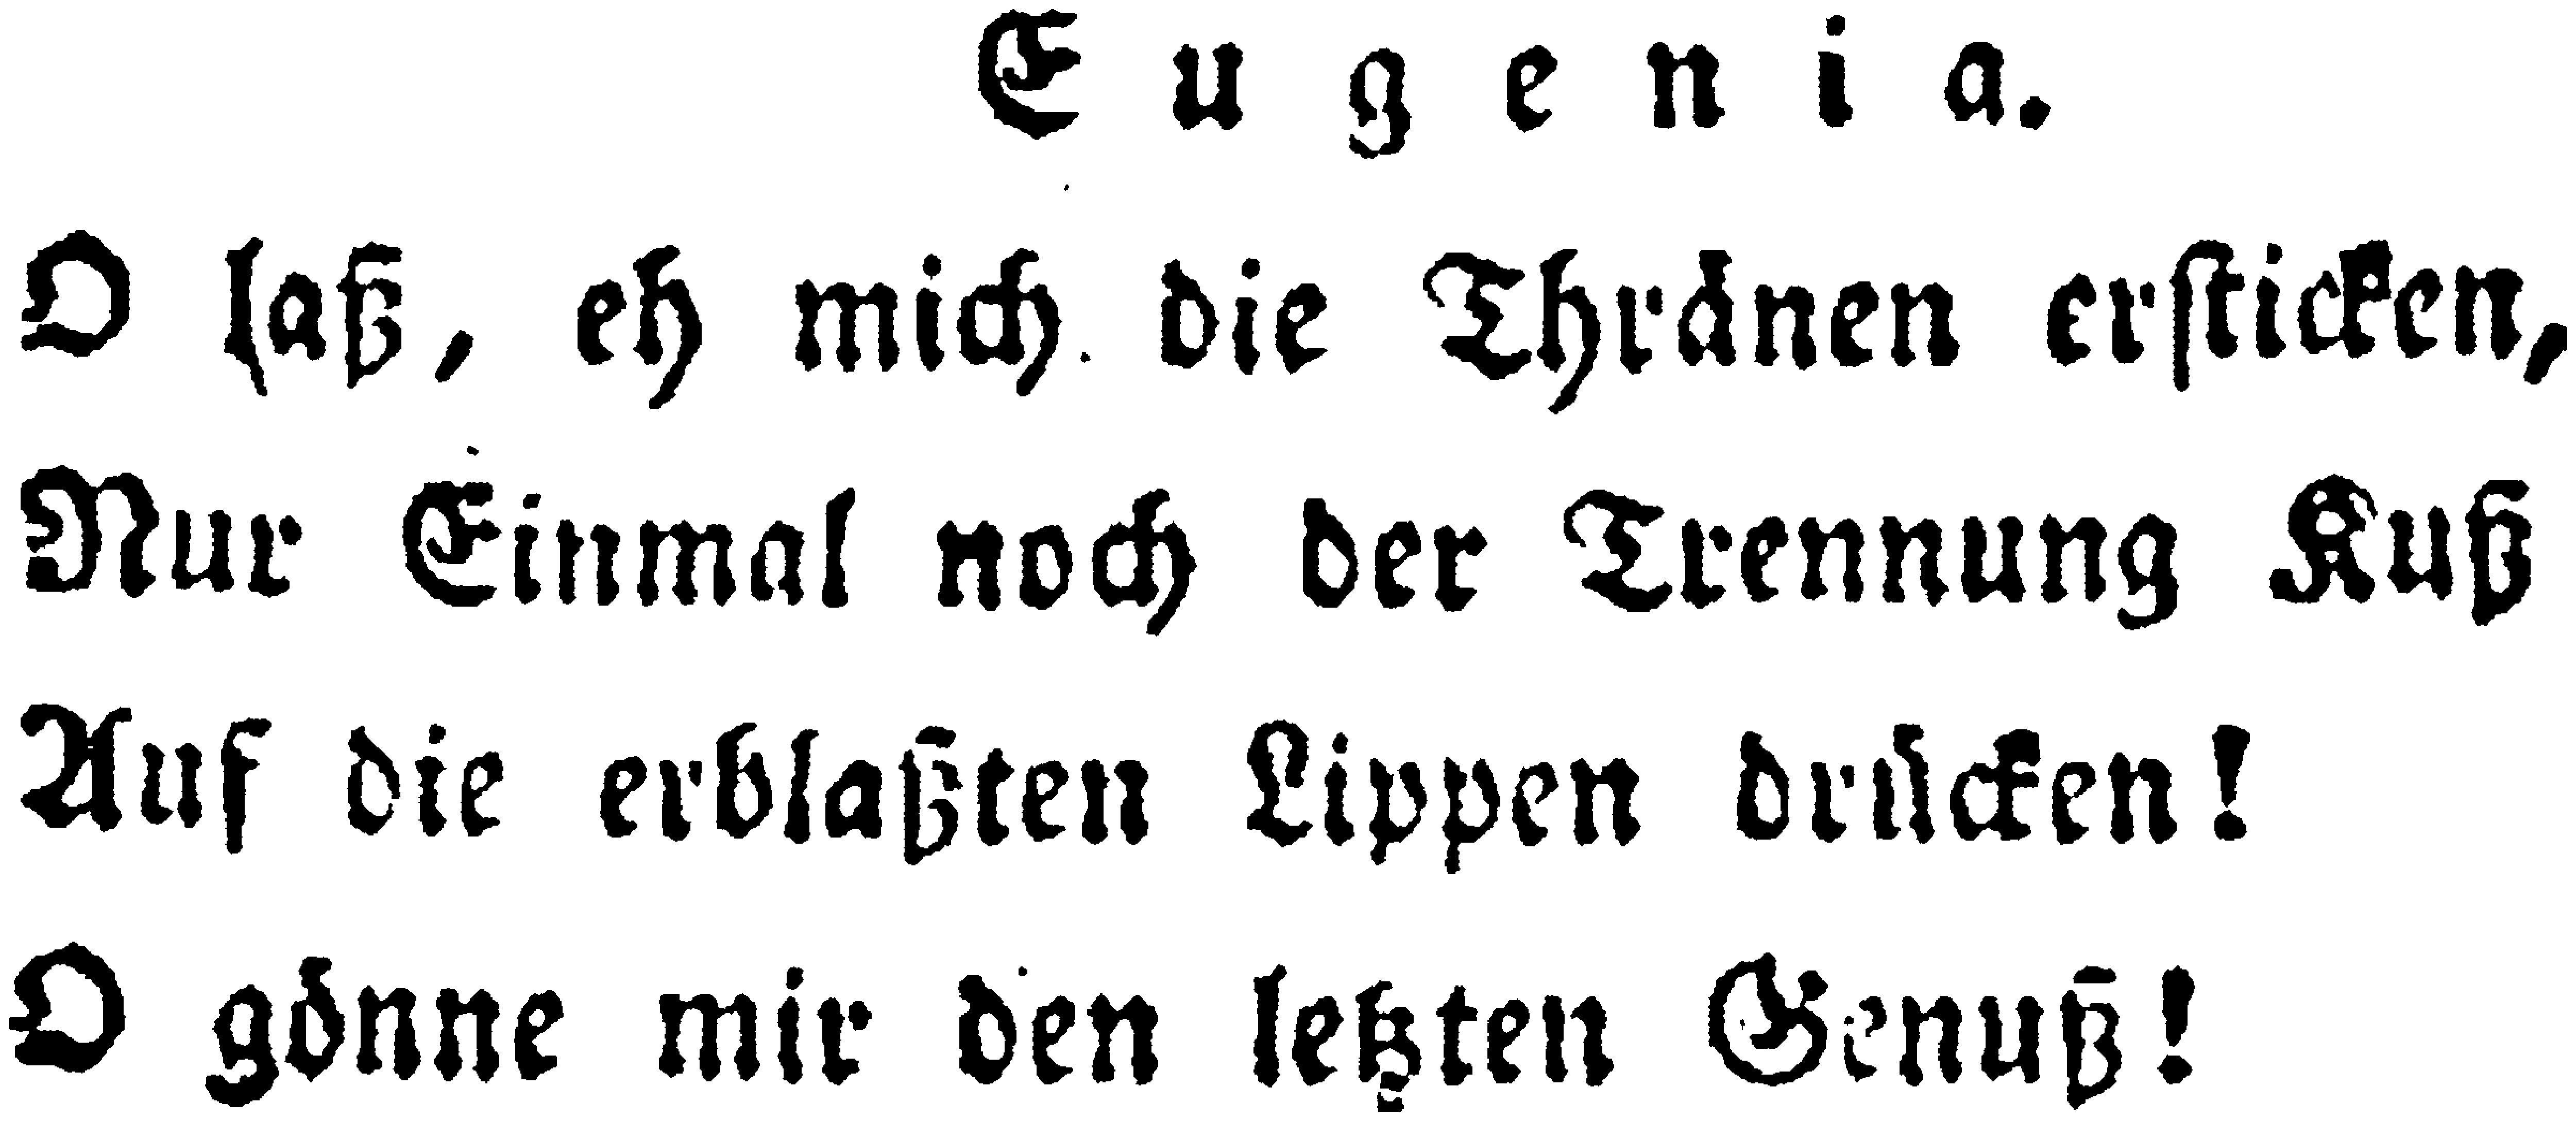
\epsfig{file=figures/example1.eps,width=\textwidth}
      \end{minipage}
      &
      \begin{minipage}{0.5\textwidth}
        E u g e n i a.\\
        O \textbf{\textcolor{bbawred}{§}}aß, eh mich die Thränen ersticken.\\
        Nur Einmal noch der Trennung Kuß\\
        Auf die erblaßten Lippen drücken!\\
        O gönne mir den le\textbf{\textcolor{bbawred}{h}}ten Genuß!
      \end{minipage}\\\\
      \texttt{Tesseract} & \texttt{OCRopus}\\
      \begin{minipage}{0.5\textwidth}
        Eugeaia.\\
        O laß, H) mich. die Tht*äaea erIHckm,\\
        Nur Einqu noch der Trennung Kuß\\
        Auf die erqußteu Lippen drückenx\\
        O gönne mie den legten Genußx
      \end{minipage}
      &
      \begin{minipage}{0.5\textwidth}
        E u g e n i a.\\
        O \textbf{\textcolor{bbawred}{h}}aß, eh mich die Thränen ersticken,\\
        Nur Einmal noch der Trennung Kuß\\
        Auf die erblaßten Lippen drücken!\\
        O g\textbf{\textcolor{bbawred}{d}}nne mir den letzten Genuß!
      \end{minipage}
    \end{tabular}
    \vspace{-2em}
\end{bbawslide}

\begin{bbawslide}{OCR-Merging: Kotzebue \enquote{Schutzgeist} (1814)}
    \begin{tabular}{cc}
    & \texttt{Merge}\\
      \begin{minipage}{0.5\textwidth}
        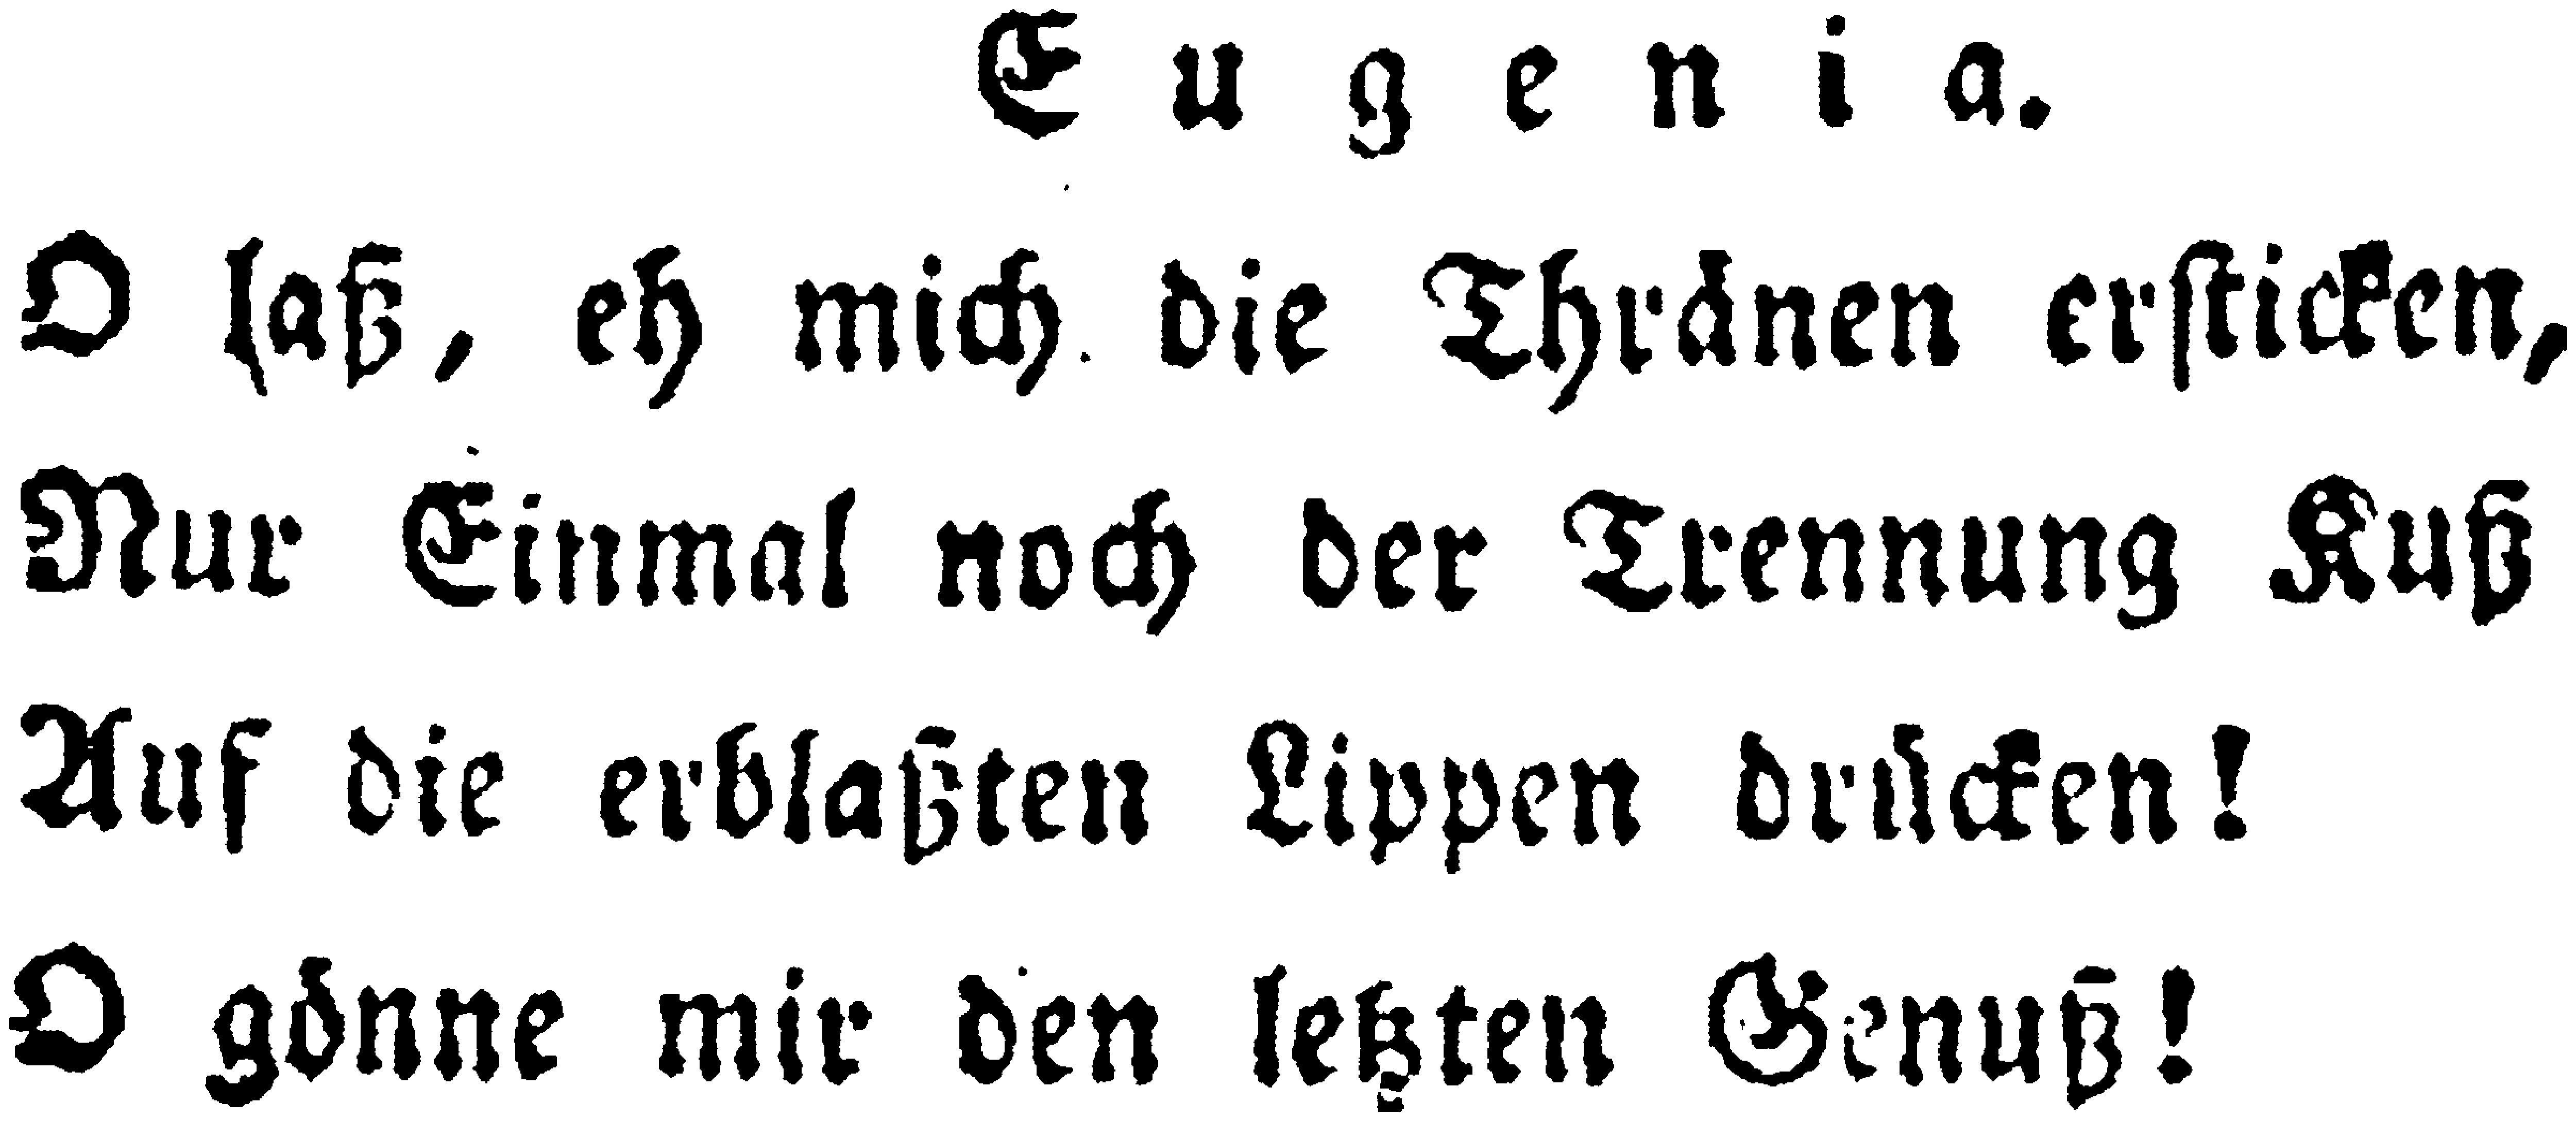
\epsfig{file=figures/example1.eps,width=\textwidth}
      \end{minipage}
      &
      \begin{minipage}{0.5\textwidth}
        E u g e n i a.\\
        O laß, eh mich die Thränen ersticken,\\
        Nur Einmal noch der Trennung Kuß\\
        Auf die erblaßten Lippen drücken!\\
        O gönne mir den letzten Genuß!
      \end{minipage}\\\\
      \texttt{Tesseract} & \texttt{OCRopus}\\
      \begin{minipage}{0.5\textwidth}
        Eugeaia.\\
        O laß, H) mich. die Tht*äaea erIHckm,\\
        Nur Einqu noch der Trennung Kuß\\
        Auf die erqußteu Lippen drückenx\\
        O gönne mie den legten Genußx
      \end{minipage}
      &
      \begin{minipage}{0.5\textwidth}
        E u g e n i a.\\
        O \textbf{\textcolor{bbawred}{h}}aß, eh mich die Thränen ersticken,\\
        Nur Einmal noch der Trennung Kuß\\
        Auf die erblaßten Lippen drücken!\\
        O g\textbf{\textcolor{bbawred}{d}}nne mir den letzten Genuß!
      \end{minipage}
    \end{tabular}
    \vspace{-2em}
\end{bbawslide}

\begin{bbawslide}{OCR-Merging: Dach \enquote{Einfältige Leichreime} (1653)}
    \begin{tabular}{cc}
    & \texttt{Abbyy Finereader}\\
      \begin{minipage}{0.5\textwidth}
        
\epsfig{file=figures/example2.eps,width=\textwidth}
      \end{minipage}
      &
      \begin{minipage}{0.5\textwidth}
        ES kostet Om kein zeitlich Gut\\
        Dns wieder zu erwerben/\\
        ES that es nicht der OpfferBluk/\\
        Cr muste selber sterben\\
        Vnd emenTod zwar/ welcher gar\\
        EinFluch vnd Grcwcl war.
      \end{minipage}\\\\
      \phantom{\texttt{Tesseract}} & \phantom{\texttt{OCRopus}}\\
      \phantom{
      \begin{minipage}{0.5\textwidth}
        Es ko\textlongs tet jhm kein zeitlich Gut\\
        Vns wieder zu erwerben/\\
        Es ihaietz?i1ichi der Opffer Blui/\\
        Er mu\textlongs te \textlongs elber \textlongs terben\\
        Vnd einenTod zwar / welcher gar\\
        EinFliich'vud Grewel war.
      \end{minipage}}
      &
      \phantom{
      \begin{minipage}{0.5\textwidth}
        Es ko\textlongs\textbf{\textcolor{bbawred}{l}}et jhm kein zeitlich Gut\\
        Vns wieder zu \textbf{\textcolor{bbawred}{t}}erwerben/\\
        Es that es nicht der Opffer Blut/\\
        Er mu\textlongs te \textlongs elber \textlongs terben\\
        Vnd einen Tod zwar/ welcher gar\\
        Ein Fluch vnd Grewel war.
      \end{minipage}
      }
    \end{tabular}
    \vspace{-2em}
\end{bbawslide}

\begin{bbawslide}{OCR-Merging: Dach \enquote{Einfältige Leichreime} (1653)}
    \begin{tabular}{cc}
    & \texttt{Abbyy Finereader}\\
      \begin{minipage}{0.5\textwidth}
        
\epsfig{file=figures/example2.eps,width=\textwidth}
      \end{minipage}
      &
      \begin{minipage}{0.5\textwidth}
        ES kostet Om kein zeitlich Gut\\
        Dns wieder zu erwerben/\\
        ES that es nicht der OpfferBluk/\\
        Cr muste selber sterben\\
        Vnd emenTod zwar/ welcher gar\\
        EinFluch vnd Grcwcl war.
      \end{minipage}\\\\
      \texttt{Tesseract} & \phantom{\texttt{OCRopus}}\\
      \begin{minipage}{0.5\textwidth}
        Es ko\textlongs tet jhm kein zeitlich Gut\\
        Vns wieder zu erwerben/\\
        Es ihaietz?i1ichi der Opffer Blui/\\
        Er mu\textlongs te \textlongs elber \textlongs terben\\
        Vnd einenTod zwar / welcher gar\\
        EinFliich'vud Grewel war.
      \end{minipage}
      &
      \phantom{
      \begin{minipage}{0.5\textwidth}
        Es ko\textlongs\textbf{\textcolor{bbawred}{l}}et jhm kein zeitlich Gut\\
        Vns wieder zu \textbf{\textcolor{bbawred}{t}}erwerben/\\
        Es that es nicht der Opffer Blut/\\
        Er mu\textlongs te \textlongs elber \textlongs terben\\
        Vnd einen Tod zwar/ welcher gar\\
        Ein Fluch vnd Grewel war.
      \end{minipage}
      }
    \end{tabular}
    \vspace{-2em}
\end{bbawslide}

\begin{bbawslide}{OCR-Merging: Dach \enquote{Einfältige Leichreime} (1653)}
    \begin{tabular}{cc}
    & \texttt{Abbyy Finereader}\\
      \begin{minipage}{0.5\textwidth}
        
\epsfig{file=figures/example2.eps,width=\textwidth}
      \end{minipage}
      &
      \begin{minipage}{0.5\textwidth}
        ES kostet Om kein zeitlich Gut\\
        Dns wieder zu erwerben/\\
        ES that es nicht der OpfferBluk/\\
        Cr muste selber sterben\\
        Vnd emenTod zwar/ welcher gar\\
        EinFluch vnd Grcwcl war.
      \end{minipage}\\\\
      \texttt{Tesseract} & \texttt{OCRopus}\\
      \begin{minipage}{0.5\textwidth}
        Es ko\textlongs tet jhm kein zeitlich Gut\\
        Vns wieder zu erwerben/\\
        Es ihaietz?i1ichi der Opffer Blui/\\
        Er mu\textlongs te \textlongs elber \textlongs terben\\
        Vnd einenTod zwar / welcher gar\\
        EinFliich'vud Grewel war.
      \end{minipage}
      &
      \begin{minipage}{0.5\textwidth}
        Es ko\textlongs\textbf{\textcolor{bbawred}{l}}et jhm kein zeitlich Gut\\
        Vns wieder zu \textbf{\textcolor{bbawred}{t}}erwerben/\\
        Es that es nicht der Opffer Blut/\\
        Er mu\textlongs te \textlongs elber \textlongs terben\\
        Vnd einen Tod zwar/ welcher gar\\
        Ein Fluch vnd Grewel war.
      \end{minipage}
    \end{tabular}
    \vspace{-2em}
\end{bbawslide}

\begin{bbawslide}{OCR-Merging: Dach \enquote{Einfältige Leichreime} (1653)}
    \begin{tabular}{cc}
    & \texttt{Merge}\\
      \begin{minipage}{0.5\textwidth}
        
\epsfig{file=figures/example2.eps,width=\textwidth}
      \end{minipage}
      &
      \begin{minipage}{0.5\textwidth}
        Es ko\textlongs tet jhm kein zeitlich Gut\\
        Vns wieder zu erwerben/\\
        Es that es nicht der Opffer Blut/\\
        Er mu\textlongs te \textlongs elber \textlongs terben\\
        Vnd einen Tod zwar / welcher gar\\
        Ein Fluch vnd Grewel war.
      \end{minipage}\\\\
      \texttt{Tesseract} & \texttt{OCRopus}\\
      \begin{minipage}{0.5\textwidth}
        Es ko\textlongs tet jhm kein zeitlich Gut\\
        Vns wieder zu erwerben/\\
        Es ihaietz?i1ichi der Opffer Blui/\\
        Er mu\textlongs te \textlongs elber \textlongs terben\\
        Vnd einenTod zwar / welcher gar\\
        EinFliich'vud Grewel war.
      \end{minipage}
      &
      \begin{minipage}{0.5\textwidth}
        Es ko\textlongs\textbf{\textcolor{bbawred}{l}}et jhm kein zeitlich Gut\\
        Vns wieder zu \textbf{\textcolor{bbawred}{t}}erwerben/\\
        Es that es nicht der Opffer Blut/\\
        Er mu\textlongs te \textlongs elber \textlongs terben\\
        Vnd einen Tod zwar/ welcher gar\\
        Ein Fluch vnd Grewel war.
      \end{minipage}
    \end{tabular}
    \vspace{-2em}
\end{bbawslide}

\begin{bbawslide}{Optimierungsoptionen: OCR-Nachkorrektur}
  \vspace*{7mm}%
  \centerslidestrue%
  \begin{itemize}
    \item auch unter optimierten Bedingungen verbleiben OCR-Fehler
    \item manuelle oder automatische Korrektur des Textes zur Erhöhung der Qualität
    \item drei Ansatzmöglichkeiten:
    \begin{itemize}\small
      \item \textbf{manuell} (Collaborative Manual Correction/ Crowdsourcing)
      \item \textbf{programmunterstützt} (Interactive Postcorrection)
      \item \textbf{automatisch}
    \end{itemize}
    \item \enquote{klassische} Aufgabe der \textbf{Computerlinguistik}
    \begin{itemize}\small
      \item Anleihen bei Rechtschreibkorrektur
      \item bzw. Schreibungsnormalisierung \hlcite{Jurish 2012}
    \end{itemize}
  \end{itemize}
\end{bbawslide}

\begin{bbawslide}{Optimierungsoptionen: OCR-Nachkorrektur}
  \vspace*{2mm}%
  \centerslidestrue%
  \textbf{Werkzeuge}
  \begin{mitemize}
    \item \textbf{manuell:}
    \begin{itemize}\small
      \item manuelle Transkription/Korrektur des OCR-Ergebnisses, erfordert umfassende Konzeption und (anfängliche) Betreuung, bietet Ansatz für Gamification
      \item diverse proprietäre und Open-Source-Lösungen, \textbf{plattformgebunden}, z.B. \texttt{DTAQ}
    \end{itemize}
    \item \textbf{programmunterstützt:}
    \begin{itemize}\small
      \item Unterstützung der manuellen Korrektur durch \textbf{Korrekturvorschläge} und Hervorhebung wahrscheinlich fehlerhafter Texterkennungsergebnisse
      \item \textbf{Po}st \textbf{Co}rrection \textbf{To}ol \url{https://github.com/cisocrgroup/PoCoTo}
    \end{itemize}
    \item \textbf{automatisch:}
    \begin{itemize}\small
      \item Korrektur auf Basis von (lexikalischen) Ground-Truth-Daten
      \item \textbf{Rechtschreibkorrekturprogramme} wie \texttt{hunspell} \url{http://hunspell.github.io/}
      \item projektspezifische (Insel)-Lösungen wie der sog. \textbf{Bremer Ansatz} für die Zeitschrift \enquote{Die Grenzboten} \hlcite{Nölte et al. 2016}
    \end{itemize}
  \end{mitemize}
\end{bbawslide}

\begin{bbawslide}{Optimierungsoptionen: Synthetisches Trainingsmaterial}
  \vspace*{7mm}%
  \centerslidestrue%
  \begin{itemize}
    \item Volltexte historischer Drucke zunehmend vorhanden
    \begin{itemize}\small
      \item manuelle Erfassung normalerweise \textbf{ohne} Text-Bild-Alignierung
      \item Erstellung von Trainingsmaterial \textbf{zeitaufwendig} und teuer
    \end{itemize}
    \item Idee: Einsatz von \textbf{Font-rendering}-Software um automatisch alignierte
          Trainingsdaten zu erzeugen
    \begin{itemize}\small
      \item Verwendung historischer Schriften, z.B.~Fraktur \url{http://www.ligafaktur.de/Schriften.html}
      \item \enquote{künstliche} Artefakte zur Nachahmung der Druckalterung
    \end{itemize}
  \end{itemize}
\end{bbawslide}

\begin{bbawslide}{Optimierungsoptionen: Synthetisches Trainingsmaterial}
  \vspace*{7mm}%
  \centerslidestrue%
  \textbf{Werkzeuge:}
  \begin{itemize}
    \item \texttt{OCRopus} (und sein Fork \texttt{Kraken}) und \texttt{Tesseract} mit \textbf{Generierungsmechanismus}
    \item viele Projekte zur Erstellung \textbf{historischer Fonts} im TTF/OTF-Format für (praktisch) alle alphabetischen Schriftsysteme
  \end{itemize}
  \begin{center}
    
\epsfig{file=figures/font_rend1.eps,width=0.8\textwidth}\\[2ex]
    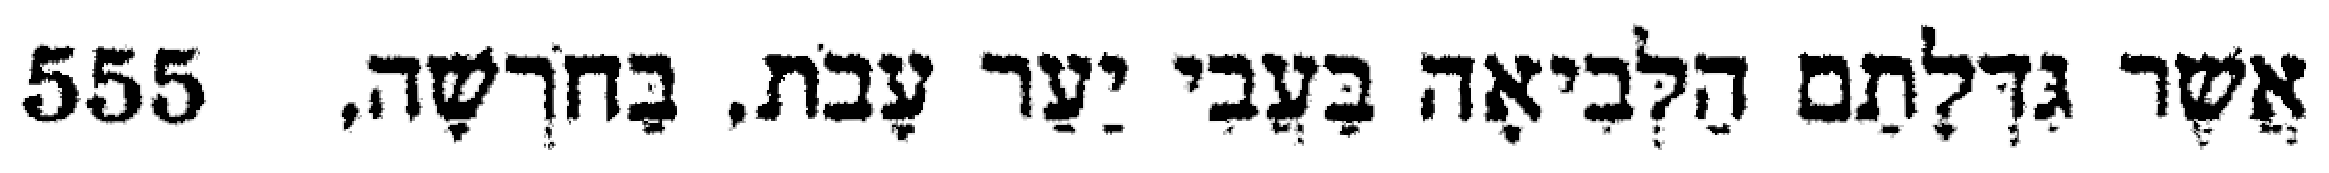
\epsfig{file=figures/font_rend2.eps,width=0.8\textwidth}
  \end{center}
\end{bbawslide}

\begin{bbawpart}{\Large\bf Komplexere OCR-Workflows}
\end{bbawpart}

\begin{bbawslide}{Komplexere OCR-Workflows}
  \vspace*{7mm}%
  \centerslidestrue%
  \begin{itemize}
    \item \enquote{einfache} OCR-Workflows in allen OCR-Lösungen implementiert
    \item \textbf{keine Möglichkeit} zur direkten Integration der diskutierten Optimierungsmöglichkeiten
    \item kein modulares \textbf{Workflowmanagmentsystem} im Bereich OCR vorhanden
    \item momentane Lösung:
    \begin{itemize}
       \item Zugriff auf \textbf{einzelne Module}
       \item Kombination in \textbf{spezifischem Workflow}
       \item aka.~Skripte und Hacks
    \end{itemize}
    \item \textbf{OCR-D}
  \end{itemize}
\end{bbawslide}

\begin{bbawslide}{Komplexere OCR-Workflows: Beispiel}
  \vspace*{2mm}%
  \begin{center}
      \epsfig{file=figures/workflow.eps,width=1.1\textwidth}%
  \end{center}
\end{bbawslide}

\begin{bbawpart}{\Large\bf OCR-D}
\end{bbawpart}

\begin{bbawslide}{OCR-D: Überblick}
  \vspace*{2mm}%
  \centerslidestrue%
  \begin{itemize}
    \item \textbf{DFG-Initiative} zur Verbesserung von OCR-Methoden für historische Drucke insbesondere
          für die Volltextdigitalisierung aller in den \emph{Verzeichnissen der im deutschen
          Sprachraum erschienen Drucke} (VD16, VD17, VD18) nachgewiesenen Exemplare
    \item \textbf{Koordinationsprojekt} an der Herzog-August Bibliothek Wolfenbüttel, der Staatsbibliothek
          Berlin, dem Karlsruher Institut für Technologie und der BBAW $\rightarrow$ Implementierung
          einer Ausschreibung für methodische
          Projekte auf allen Ebenen eines optimierten OCR-Workflows
    \begin{itemize}\small
      \item Bildvorverarbeitung
      \item Layoutanalyse
      \item Texterkennung/-optimierung
      \item Modeltraining
      \item Langzeitarchivierung
      \item Qualitätssicherung
    \end{itemize}
  \end{itemize}
\end{bbawslide}

\begin{bbawslide}{OCR-D: Projektprämissen}
  \vspace*{7mm}%
  \centerslidestrue%
  \begin{itemize}
    \item \textbf{Lückenschluss} zwischen Forschung und Praxis
    \begin{itemize}\small
      \item Transfer der Forschungsergebnisse
      \item zugängliche und nachnutzbare Implementierungen
    \end{itemize}
    \item \textbf{Methodenpluralismus}
    \begin{itemize}\small
      \item insbesondere bei schwierigen Vorlagen: \textbf{kein} bester Algorithmus
      \item Implementierung möglichst \textbf{vieler Ansätze} samt \enquote{Auswahlmechanismus}
    \end{itemize}
    \item konsequent \textbf{Open-Source}
    \begin{itemize}\small
      \item Veröffentlichung des Quellcodes \textbf{und}
      \item Anschluss an vorhandene Communities
    \end{itemize}
  \end{itemize}
\end{bbawslide}

\begin{bbawslide}{OCR-D: Open-Source-Paradigma}
  \vspace*{2mm}%
  \centerslidestrue%
  \begin{itemize}
    \item öffentlich geförderte Projekte $\leadsto$ öffentlich verfügbare Projektergebnisse
    \item dank \textbf{Digital Humanities} \enquote{Kulturrevolution}
    \begin{itemize}\small
      \item Daten (i.e.~Texte) veröffentlicht unter CC
      \item \enquote{Belohnung} durch wissenschaftliche Veröffentlichung und Zitierungen
      \item \textbf{reproducible science}
    \end{itemize}
    \item im Bereich der Werkzeuge: \textbf{Verbesserungsbedarf}
    \begin{itemize}\small
      \item Entwicklung von Tools mit hohem Aufwand und öffentlich gefördert
      \item am Projektende Veröffentlichung eines Archivs mit Quellcode unter Open-Source-Lizenz
    \end{itemize}
    \item Ziel: Einbindung der Nutzercommunity von \textbf{Anfang an}
    \begin{itemize}\small
      \item Fehlermeldung und Funktionalitätsfeedback während der Entwicklung
      \item Weiterentwicklung und Pflege auch nach Ablauf der Förderung
    \end{itemize}
  \end{itemize}
\end{bbawslide}

\begin{bbawslide}{OCR-D: Open-Source-Paradigma}
  \vspace*{2mm}%
  \begin{center}
      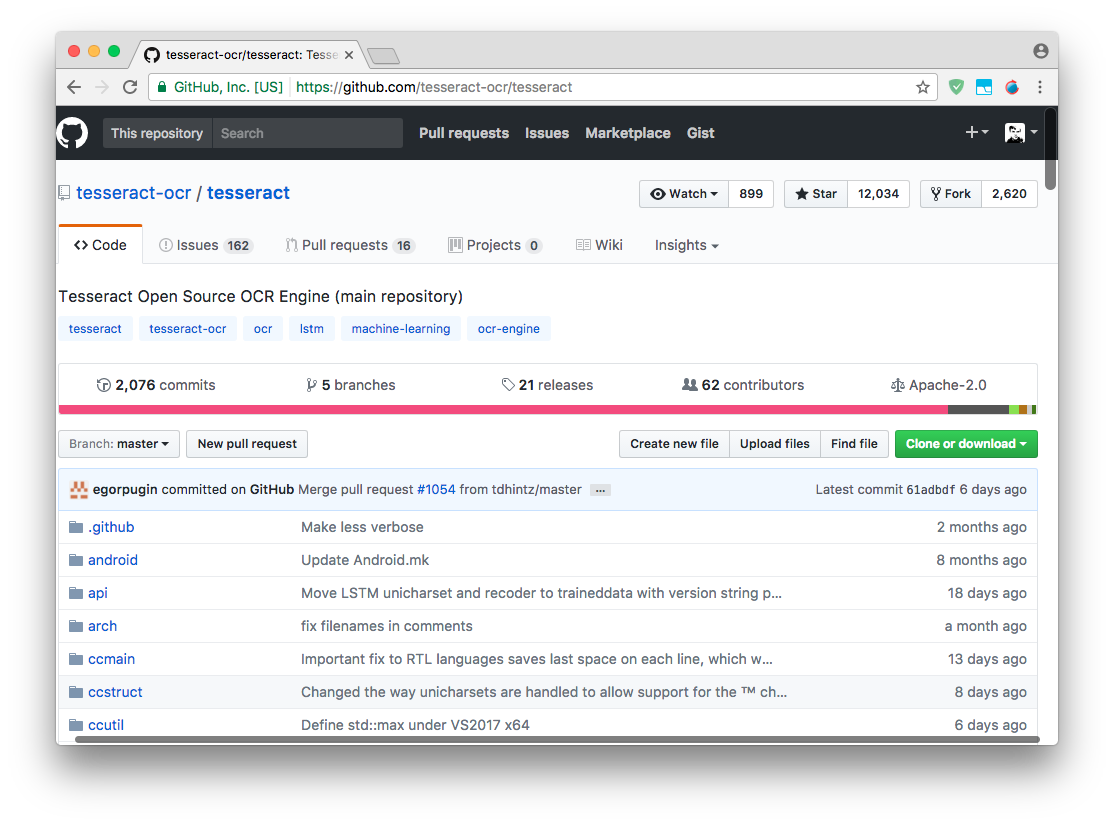
\epsfig{file=figures/tesseract_screen.eps,width=0.8\textwidth}%
  \end{center}
\end{bbawslide}

\begin{bbawpart}{\Large\bf Danke für Ihre Aufmerksamkeit!\\}
OCR-D-Team: Elisa Hermann, Maria Federbusch, Clemens Neudecker, Ajinkya Prabhune, \textbf{Matthias Boenig}\\
Mehr zu OCR: \url{https://www.zotero.org/groups/ocr-d}
\end{bbawpart}

\end{document}

%\begin{bbawpart}{\Large\bf Warum braucht man OCR?}
%\end{bbawpart}

%\begin{bbawslide}{Warum braucht man OCR?}
%  \vspace*{7mm}%
%  \centerslidestrue%
%  \begin{itemize}
%    \item
%  \end{itemize}
%\end{bbawslide}

%
% modelines
%

%%% Local Variables:
%%% mode: LaTeX
%%% coding: utf-8
%%% tab-width: 2
%%% indent-tabs-mode: nil
%%% End:

% vim: set ts=2 sw=2 expandtab :
